\documentclass[11pt,a4paper]{article}

% ===== Packages =====
\PassOptionsToPackage{numbers,sort&compress}{natbib}

\usepackage[T1]{fontenc}
\usepackage{newtxtext,newtxmath}
\usepackage{amsmath,amsfonts,bm}
\usepackage{graphicx}
\usepackage{booktabs,multirow,array}
\usepackage{caption,subcaption}
\usepackage{algorithm2e}
\usepackage{relsize}
\usepackage[margin=2.5cm]{geometry}
\usepackage{setspace}
\usepackage[dvipsnames]{xcolor}
\usepackage[hyphens]{url}
\usepackage{natbib}  
\usepackage{comment}


% ===== Proposition Environment =====
\newtheorem{proposition}{Proposition}
\newtheorem{lemma}{Lemma}
\newtheorem{proof}{Proof}
\newtheorem{hypothesis}{Hypothesis}
\newtheorem{definition}{Definition}

\DeclareMathOperator*{\argmin}{arg\,min}

\renewcommand{\topfraction}{0.75}  
\renewcommand{\bottomfraction}{0.75} 
\renewcommand{\textfraction}{0.2} 

\begin{document}

% ===== Title and Authors =====
\title{A library with rabbit holes: an information space where serendipity can be sought}
\author{
    Tatsuya Kanatsu\textsuperscript{1}, Tohru Iwasaki\textsuperscript{2}, Hideaki Ishibashi\textsuperscript{1}, \\
    Kaori Yoshida\textsuperscript{1}, and Tetsuo Furukawa\textsuperscript{1} \\[3pt]
    \small \textsuperscript{1}Graduate School of Life Science and Systems Engineering, Kyushu Institute of Technology, Japan \\
    \small \textsuperscript{2}Data / AI System Division, ZOZO, Inc., Japan \\
    \small Corresponding author: furukawa@brain.kyutech.ac.jp
}
\date{}
\author{} % Remove the author name from the title page
\maketitle

\begin{abstract}\noindent
    Serendipity cannot be searched for: no one can name in advance what would
    count as finding it. What one can do is explore, as visitors to a library
    always have. This paper asks what an information space must hold if
    serendipity is to be sought, and answers with a concept: a library
    with rabbit holes. Its floors arrange works by denotation, genre above
    all; through them run \textit{rabbit holes}, vertical passages crossing
    genres while holding fixed a \textit{connotative} closeness no
    single word carries. An explorer may leap through one onto another floor
    whenever they wish---the finding, if any, is their own. Such an exploration
    space is a matter of information \textit{representation}: the layer any
    interface presupposes and none can substitute for. What is needed is a
    \textit{disentangled} representation, separating the denotative
    from the connotative. Once the scope of the data is fixed, an inductive
    bias follows naturally: \textit{optimal transport}. Among the infinitely
    many representations fitting the same data, the \textit{Optimal
        Transport Fiber Bundle (OT-FB)} is essentially unique yet learnable from
    real data. What the bundle says about rabbit holes: a hole is determined
    by how one genre stands to another as a whole. Neither a label nor the
    affinity of any two works reaches a relation of that scale. A coordinate
    reaches it: naming nothing, it marks a place within the whole
    arrangement of works. Such signposts are what the seeker needs: in
    this space, what cannot be searched for can be sought.
\end{abstract}

\begin{quote}\parindent=0pt\parskip=.5em\noindent
    \begin{center}
        \textbf{Structured Abstract}
    \end{center}
    \textbf{Purpose.}
    Serendipity cannot be searched for: what would count as finding it cannot
    be named in advance. What remains is exploration. This paper asks what an
    information space must hold if serendipity is to be sought in it---a
    question of information \textit{representation}.

    \textbf{Design/methodology/approach.}
    We propose a concept: a library with \textit{rabbit holes}---a
    \textit{disentangled representation} of the entangled data space.
    Its floors arrange works by denotation, genre above all; rabbit holes
    run vertically through the floors, crossing genres while holding
    fixed a connotative closeness no single word carries. Once disentangled,
    an explorer can move within a genre or leap through a rabbit
    hole into another, both by intent.

    \textbf{Findings.}
    Under a natural inductive bias---\textit{optimal transport}---the
    disentangled representation takes a definite form: the \textit{Optimal
        Transport Fiber Bundle (OT-FB)}, essentially unique among the
    infinitely many representations fitting the same data, and learnable
    from real data. What it says about rabbit holes: a hole is determined
    not by what two works share, but by how one genre stands to another as
    a whole.

    \textbf{Originality/value.}
    The paper makes three contributions. It locates the design of an
    exploration space in representation rather than interface. It gives
    that representation a definite form, essentially unique yet learnable
    from data. And it explains a limit long attested in indexing practice:
    a name attaches to one work at a time, while connotation lives in how
    whole genres stand to one another. A coordinate, naming nothing,
    carries it---and by such signposts, what cannot be searched for can be
    sought.
\end{quote}

\noindent\textbf{Keywords:}
serendipity, exploratory search, information representation,
disentangled representation, optimal transport, fiber bundle


%%%%% Section 1 Introduction %%%%%
\section{Introduction}\label{sec:introduction}

A visitor comes to the reference desk of a music library.

\begin{quote}
I am looking for something like Miles Davis---that atmosphere I cannot
quite name.
\end{quote}

The librarian asks for something more specific. The visitor searches for
words, falls silent for a while, and finally offers:

\begin{quote}
Quiet, but with feeling in it; impressionistic; colours that seem to melt
into one another\ldots{} I cannot say it well.
\end{quote}

A visitor who gets this far is doing well; most never move past the first
sentence. The librarian understands the request---or feels she does. But
consider what the catalogue gives her to work with. From ``Miles Davis'' it
retrieves a genre (jazz), an instrument (trumpet), a period (the 1950s and
60s), a country (the United States). A search on these facets returns hard
bop, fusion, and a quantity of other trumpeters, most of it not what the
visitor wants. Some weeks later, by another route---browsing a shelf, or a
friend's recommendation---he comes upon Debussy's piano music, and thinks:
\emph{so this is what I was looking for.}

This scene is our point of departure, and we take it apart before building
on it. First, everything the catalogue records has changed. Jazz has become
classical, trumpet piano, the 1950s the 1900s, America France; a performer
has even become a composer. Not one catalogued attribute survived the
passage---and yet the visitor's criterion was met. Second, the affinity is
not a private fancy. The kinship between the music around Miles Davis and
impressionist harmony has been remarked many times: the modal language of
\emph{Kind of Blue}, Bill Evans's pianism, and Gil Evans's orchestration
have all been discussed in relation to Debussy and
Ravel~\cite{TODO-musicology}. What the visitor sensed lies \emph{in the
works}; it is simply written in none of the catalogue's fields. Third, what
the visitor discovered was not a piano piece. He did not say ``what a fine
piece''; he said ``this is what \emph{I} was looking for.'' The object of
his discovery was his own criterion---something he could not have stated
before the encounter. Fourth, he had indicated his need in two ways: by
pointing at a work (``like Miles Davis''), and by heaping up partially apt
words (``quiet, with feeling, melting colours''). Neither is a subject
term, and the catalogue has a field for neither.

Wilson distinguished two powers at which bibliographic control can
aim~\cite{Wilson1968}: \emph{descriptive} power, the power to find
everything that bears on a topic, and \emph{exploitative} power, the power
to put recorded knowledge to one's own best use. What the cataloguing
tradition built to a high finish---from Cutter's objects through facet
analysis---is the former; the latter has been left, for the most part, to
the skill of readers and librarians. Our visitor is asking for the latter:
not what a work is \emph{about}, but how it \emph{feels}.

Two kinds of attribute must therefore be told apart, and the pair will
anchor everything that follows. \emph{Denotative} attributes can be
expressed as sets of mutually exclusive labels and implemented as facets:
genre, period, creator, instrument, country. \emph{Connotative} attributes
cannot. They resist a single name, come in degrees, are many-dimensional,
interfere with one another, and take form in the encounter between work and
listener. What Miles Davis and Debussy share is of this second kind. Cross
the pair with the familiar division between known-item search and
exploratory browsing, and four quadrants appear
(Table~\ref{tab:quadrants}). Faceted navigation is exploratory yet entirely
denotative, so the customary opposition of ``facets versus exploration''
misses the point: what facets fail to carry is not exploration but the
unnamed. And the quadrant of connotative search---retrieving a work by a
quality no one can name---is nearly empty. Why it is empty will become
clear in Section~\ref{subsec:third}.

\begin{table}[t]
\centering
\caption{Two kinds of attribute crossed with two modes of seeking.}
\label{tab:quadrants}
\begin{tabular}{lll}
\toprule
 & Known-item search & Exploratory browsing \\
\midrule
Denotative  & bibliographic search, OPAC & faceted navigation \\
Connotative & (nearly empty) & readers' advisory, Book House \\
\bottomrule
\end{tabular}
\end{table}

This problem is not new to library and information science. It has been
worked on from three directions, by three lineages that rarely cite one
another. How ``quiet, with feeling, melting colours'' might be written into
a bibliographic record is a question of \emph{representation}
(Section~\ref{subsec:first}). That the visitor could not say what he sought
until he had found it is a question about \emph{the seeker}
(Section~\ref{subsec:second}). How a system might receive ``like Miles
Davis'' is a question about \emph{the means of access}
(Section~\ref{subsec:third}). Section~\ref{sec:lineages} follows each
lineage to its endpoint; laid over one another, the three endpoints
determine what is required almost uniquely. It is not another interface. It
is a \emph{representation}---something written into records, outliving its
maker, shared across libraries---for qualities that have no name; for no
interface can surface what the representation beneath it does not already
encode~\cite{Blair1985289,Furnas1987964}. Section~\ref{sec:framework}
states the proposal: a coordinate system in which a work's nameable
properties and its unnamed qualities occupy separate coordinates, the
unnamed ones serving as \emph{headings without names}---and there
serendipity, too, acquires a precise sense: the seeker's recognition that
one of their own unnamed targets is expressed by such a coordinate.
Section~\ref{sec:mathematics} supplies the mathematics on which the
proposal leans---the metric under which the coordinate system is unique, so
that whoever computes it obtains the same one; this, we will argue, is the
condition for coordinates to serve as authority data.
Section~\ref{sec:computation} shows that the coordinates can be learned
from a collection and its catalogue metadata,
Section~\ref{sec:demonstration} demonstrates this on real data,
Section~\ref{sec:discussion} discusses what changes for libraries, and
Section~\ref{sec:conclusion} concludes.

%%%%% Section 2 Three lineages %%%%%
\section{Three lineages}\label{sec:lineages}

The scene touches three questions at once, and the field has pursued all
three: how such qualities might be represented, what the seeker is
seeking, and how works might be reached. Three lineages---which seldom
cite one another. What follows is not a survey of any of them. We put one
question to all three, and follow each only as far as its answer. A thing
this field learns can end up in two places: in the \emph{record}, where it
outlives its maker and travels between libraries---call this a
\emph{representation}---or in the session, the interview, the interface,
the librarian's own skill, where it works and then vanishes---call this an
\emph{interface}. The question, then: \emph{what did each lineage learn,
and where did the learning end up?}

%%%%%%%%%%%%%%%%%%%%%%%%%%%%%%%%%%%%%%%%%%%%%%%%
\subsection{The first lineage: representing what has no name}
\label{subsec:first}

The instrument of this lineage has been the name. Facet analysis divides a
domain by named characteristics into classes that are mutually exclusive
and jointly exhaustive, and the field's standards share the commitment:
definition by properties is preferred, definition by enumeration admitted
only where the enumeration is closed~\cite{ISO704}. For most of what a
catalogue does, the instrument serves.

The visitor said ``impressionistic'', and the word shows exactly where it
stops serving. Debussy is routinely classed under \emph{Impressionism};
had the librarian taken the word as a genre term, she would have reached
the answer---and the label would have excluded Miles Davis, the very work
the visitor started from. A label that expels the seeker's own point of
departure is no expression of his criterion. Sharpen the label and members
fall out; widen it and noise floods in; either way, what the seeker had
encircled is gone. We will call this \emph{flattening by labelling}: the
phenomenon has no established name of its own, though Olson's \emph{power
to name} comes close~\cite{Olson2002}. Nor is it an accident of poor
vocabulary design. The limit was identified from within the lineage
itself. Wilson showed that even a document's \emph{subject}---the
supposedly firm ground---is indeterminate~\cite{Wilson1968}; and Mai, in
the lineage's sharpest formulation, concluded that indexing

\begin{quote}
is not a neutral and objective representation of a document's subject
matter but the representation of an interpretation of a document for
future use~\cite{Mai2001591}.
\end{quote}

On his Peircean account, interpretation is an unlimited chain of signs; a
label halts the chain at a point the indexer chooses. The empirical record
concurs: agreement between indexers on such qualities is persistently
low---in a classic test with images, thirty-nine indexers agreed on terms
at an average of seven per cent~\cite{Markey1984155}---and Shatford Layne
judged the abstract layer of images, where mood and atmosphere fall,
impossible to index ``with any consistency'', while insisting that it
should not therefore be abandoned~\cite{ShatfordLayne1994583}. One may
read these numbers darkly, as proof that connotative attributes cannot be
measured at all. We leave that question open here;
Section~\ref{sec:framework} answers it.

What form remains, if not the name? Pejtersen, analysing recorded
conversations of fiction readers with librarians, found their criteria to
be ``a combination of several different features''---never a single
dimension~\cite{Pejtersen1983230}. And the set that satisfied our visitor,
\{the recordings around Miles Davis, Debussy's piano works, \ldots\},
shares no facet value at all, yet coheres. There is a formal name for such
a set: a \emph{polythetic class}, whose members share many attributes
pairwise while no single attribute runs through the
whole~\cite{Needham1975349}. The expression the visitor needs is
extensional---the set itself, shown rather than described. But precisely
here the lineage stops: extensional definition is admitted only as closed
enumeration, and this set is not closed. Recordings not yet heard, works
not yet written, belong to it. \emph{The lineage learned the right
form---an open extension---and possessed no way to write one into a
record.}

%%%%%%%%%%%%%%%%%%%%%%%%%%%%%%%%%%%%%%%%%%%%%%%%
\subsection{The second lineage: serendipity and the unnameable need}
\label{subsec:second}

What happens at the moment the visitor thinks, \emph{so this is what I was
looking for}? The classical answer belongs to Merton:

\begin{quote}
The serendipity pattern refers to the fairly common experience of
observing an unanticipated, anomalous and strategic datum which becomes
the occasion for developing a new theory or for extending an existing
theory~\cite{Merton1948505}.
\end{quote}

Look closely at what the unexpected datum occasions: not a new fact about
the world, but a reformulation of the observer's own theory. The surprise
comes from outside; what changes is inside. Merton's serendipity was
reflexive at its origin---and the scene reproduces the structure exactly.
What the visitor gained was not knowledge of Debussy but knowledge of his
own criterion, which had existed, unverbalized, all along.

LIS has built a vigorous research tradition on serendipity, and to it we
put our one question: where has the discovered thing been placed? Foster
and Ford moved serendipity from happy accident to something arising from
the seeker's own conditions and strategies~\cite{Foster2003321}; Erdelez
gave the unexpected finding of information a name and a
research programme~\cite{Erdelez1999}; Makri and Blandford resolved the
experience into unexpectedness, insight and
value~\cite{Makri2012part1,Makri2012part2}. Each sharpened the
phenomenon's structure. Yet in each, what is discovered is placed in the
world---information, works, connections. Describe our scene in these terms
and everything fits; but the one fact that mattered, that the visitor
learned his own criterion, falls out of the description. Merton's
reflexive structure was not inherited.

The same field holds a second stream, one that made unnameability its
explicit subject---and the two streams hardly cite each other. Taylor
distinguished four levels of an information need: visceral, conscious,
formalized, compromised~\cite{Taylor1968178}. The scene is his textbook
case: ``that atmosphere I cannot quite name'' is visceral; the three
groped adjectives are the move to conscious; and what is finally typed
into the catalogue---``jazz'', ``trumpet'', ``1950s''---is compromised,
the need pared down at every step. The anomalous-state-of-knowledge
hypothesis went further: a need of this kind cannot, in principle, be
specified by its owner, and the system should therefore not demand a
specification~\cite{Belkin198261}---by which light the librarian's
``something more specific, please'' was precisely the wrong request.
Kuhlthau placed the formation of a focus inside the search process rather
than before it~\cite{Kuhlthau1991361}; behavioural decision research found
preferences \emph{constructed} in the course of elicitation rather than
revealed by it~\cite{Slovic1995364}.

Join the two streams, and a conclusion follows at once. If the need cannot
be named in advance, its satisfaction cannot be a matching---there is
nothing to match against. It can only be \emph{recognition after the
encounter}. The visitor does not know, until Debussy, precisely what he
was seeking; at the encounter, he knows. In connotative access, then,
serendipity is not a peripheral accident: it is the normal mode in which
criteria are discovered. \emph{The lineage learned that the target is
recognized rather than specified---and kept placing the recognized thing
outside the seeker, in the world.}

%%%%%%%%%%%%%%%%%%%%%%%%%%%%%%%%%%%%%%%%%%%%%%%%
\subsection{The third lineage: reaching without naming}
\label{subsec:third}

The traditional mode of access is predicative: the user states a term, and
the system returns what was described by it. Its premises---that the user
can say the word, and that the work carries it---fail twice in our scene.
But the visitor showed the other mode himself, untaught: ``like Miles
Davis'' is not a predication but an act of pointing. Retrieval research
formalized this as \emph{ostensive access}, the query as a growing set of
indicated exemplars~\cite{Campbell1996251}; Pejtersen's Book House let
readers search by icons rather than words~\cite{Pejtersen1983230}.
Pointing adds no label, so it cannot flatten. And the scene shows why the
exemplars must be several: ``like Miles Davis'' alone leaves undecided
which of that music's dozens of properties is meant---the trumpet, the
modal harmony, the decade, the quiet---and only when Debussy is added do
genre, instrument and period fall away.

Then one limit decides everything: an ostensive query cannot be recorded.
Suppose the librarian had known the Miles--Debussy kinship. She could have
answered on the spot---but where in the record could she have written that
knowledge down? No field receives it. It leaves when she leaves, and the
next visitor gropes for words from the beginning. An institution is
precisely the practice of writing things down so that they can be handed
on; what cannot be recorded may live as personal skill, but it does not
accumulate. Here is why the connotative quadrant of
Table~\ref{tab:quadrants} stands nearly empty---not conceptual
impossibility, but infrastructure. Bibliographic records describe items
one at a time; ostension requires similarity \emph{between} items. The
tradition built collocation by author and by
subject~\cite{Cutter1876}; it did not build collocation by connotative
likeness. Did not---which is not the same as could not.

Could the similarity itself be computed from the works? Two routes were
tried. On the first, the analyst names a quality and prescribes its
formula: readability from sentence lengths~\cite{Flesch1948221}, texture
from six named features~\cite{Tamura1978460}, musical mood from named
parameters mapped onto adjectives~\cite{Hevner1936246}. The route failed
systematically---it demands that dimensions be named in advance, and
naming is what these qualities resist; Tamura and colleagues said as much
themselves, finding ``fundamental problems in digital analysis of
textures''. On the second route, dimensions are derived rather than named:
multidimensional scaling recovers a space of nearness from similarity
judgments alone~\cite{Shepard1962125}, and latent semantic indexing
condenses the term--document matrix into factors that are, in principle,
unnamed~\cite{Deerwester1990391}. The watershed, note, is not machine
learning. The vector space model had documents as feature vectors by
1975~\cite{Salton1975613}; but its dimensions were words, and connotation
does not live in single words---it lives in patterns of their
distribution, which is what the latent factors recover. Modern embeddings
continue this route rather than break with it. And within the same route
lies a mechanism this paper will lean on: from a \emph{set} of relevant
documents, a \emph{distribution} can be estimated~\cite{Lavrenko2001120}.
A set goes in; a rule of judgment comes out; and the rule is open, passing
verdicts on documents not yet seen.

The newest chapter was written mostly outside libraries. The road most
travelled to ``something like Miles Davis'' now runs through a streaming
service, whose collaborative filtering never looks at the works at all: it
factorizes the record of who listened to what, deriving a stand-in for
connotative proximity from the behaviour of other users. It works. But
consider the coordinate system it yields. It is free up to rotation, so
the same data admit infinitely many equivalent systems and nothing in the
mathematics prefers one; it shifts when its user population shifts; and it
cannot be written into a bibliographic record or shared across libraries.
\emph{The lineage learned to reach without naming---by pointing, by
deriving, by proxy---and everything it built took the form of an
interface. What it never produced is a representation.}

%%%%%%%%%%%%%%%%%%%%%%%%%%%%%%%%%%%%%%%%%%%%%%%%
\subsection{Where the lineages meet}\label{subsec:meet}

Now lay the three endpoints over one another.

The first lineage asks for an open extension and cannot write one down.
The third holds the mechanism that repairs this at a stroke: derive a
distribution from the set, and the enumeration opens---the distribution
judges recordings not yet heard, expressing what the members share without
ever saying it. And a distribution can be indicated by a \emph{position}.
A position can be written down. At that moment, what was an interface
becomes a representation. The knowledge our librarian had nowhere to put
acquires a place in the record: not as a name, but as a position. The
empty quadrant fills.

The second lineage dictates how such positions must be found. The seeker
cannot state coordinates---that would demand a formalized need from a
visceral one, the very demand ruled out above. A position can only be
narrowed the way the visitor narrowed his: through encounter, and
recognition. And this, the lineage showed, is no makeshift but the only
way.

At the intersection, what the second lineage left unclaimed is recovered.
What the visitor recognized in Debussy was not the piece; the piece was
the occasion. What he recognized was that his target is expressed \emph{as
this position}. That is Merton's reflexive structure, expressible at last
in the form the other two lineages supply. The next section states it as a
proposal.

%%%%% Section 3 A Library with Rabbit Holes %%%%%
\section{A Library with Rabbit Holes}\label{sec:framework}

Recall the visitor introduced in Section~\ref{sec:introduction}. Part of what he
wants he can clearly name---a performer (Miles Davis), a work (\textit{Kind of
    Blue}), and with them a genre (jazz)---and for that part, any catalogue serves.
The rest he could only circle with words: quiet, with feeling in it, colors
melting into one another. That part is connotative, and it belongs not to search
but to exploration. What exploration space, then, does such a visitor need? That
question is the subject of this section.

Throughout this paper, a collection is taken to give us two kinds of data:
\emph{descriptors}, the structured names carried on the bibliographic record,
and \emph{content data}, vectorial data representing the work itself, equipped
with a general-purpose inner product by which the closeness of two works is
measured. We call the pair \emph{collection data}; it is all we have to build
from. We keep, unless otherwise stated, to the simplest case, in which the only
descriptors given are genre and title.

\begin{figure}[t]
    \centering
    \begin{subfigure}{0.51\linewidth}
        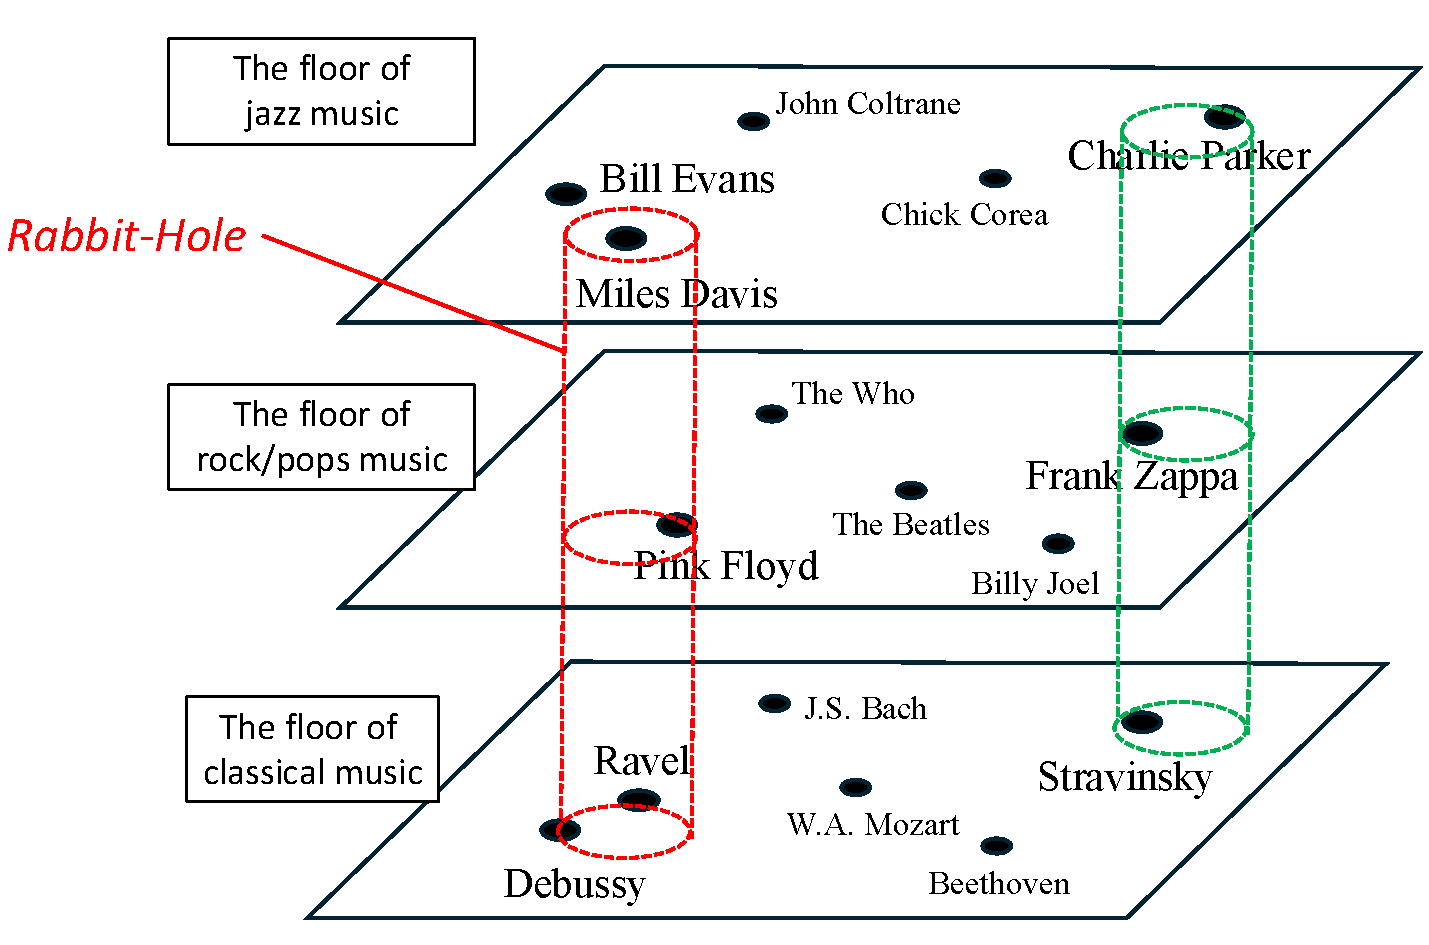
\includegraphics[width=1.0\linewidth]{fig/fig1a.pdf}
        \caption{The multi-floor library with rabbit holes (disentangled view).}
    \end{subfigure}
    \vspace{3mm}
    \begin{subfigure}{0.48\linewidth}
        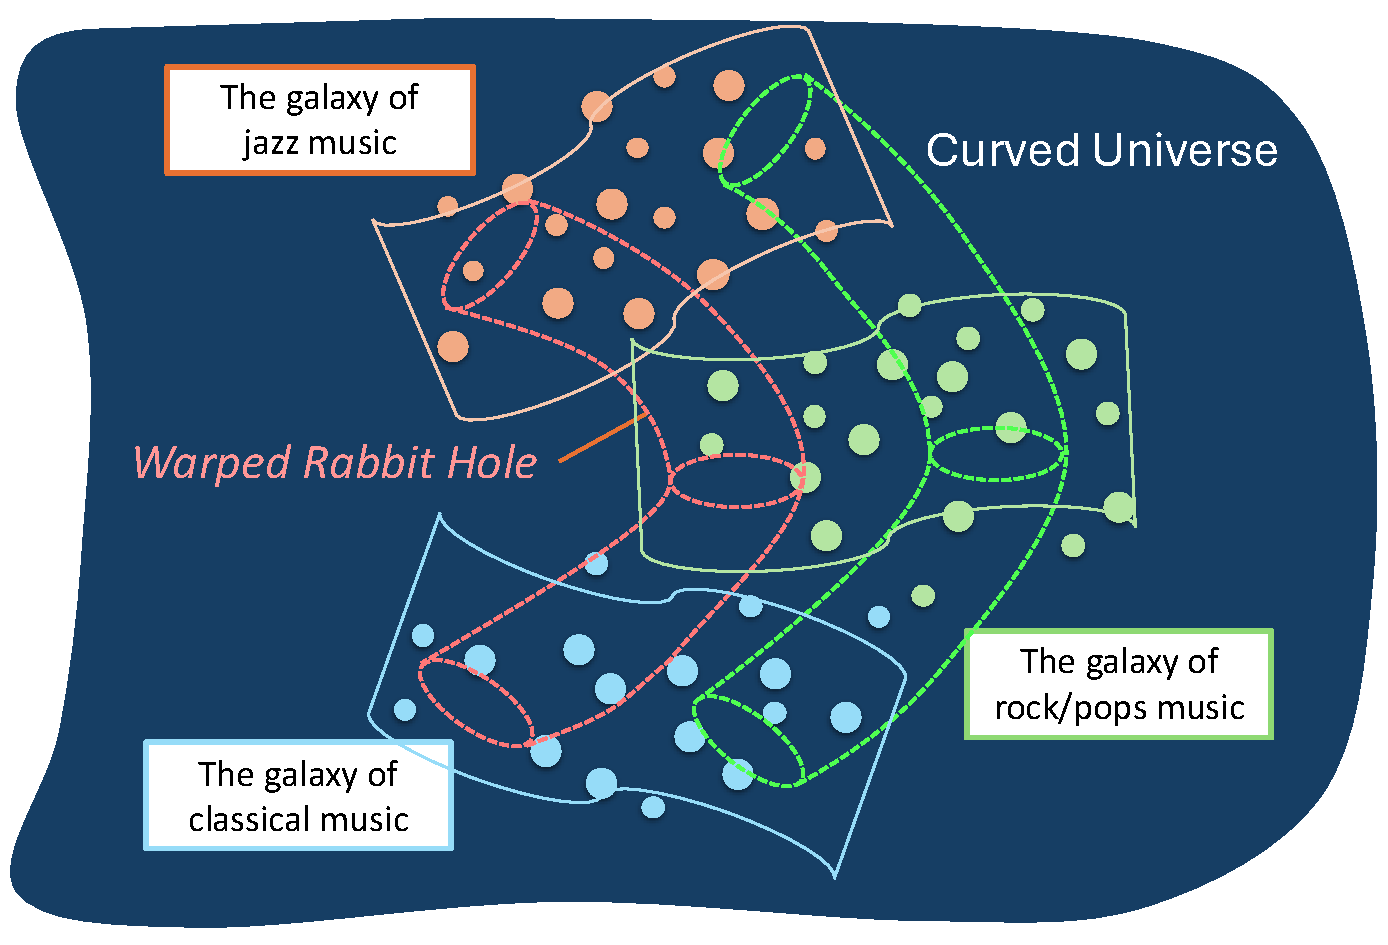
\includegraphics[width=1.0\linewidth]{fig/fig1b.pdf}
        \caption{The multi-galaxy curved universe (entangled view).}
    \end{subfigure}
    \caption{
        \textbf{Two views of one representation.}
        (a) The multi-floor library: each floor holds one genre, works
        within a floor are arranged by connotative closeness, and
        \textit{rabbit holes} run vertically, opening at the same
        connotative position on every floor. Each point is a work,
        labelled by its artist for legibility; two holes are drawn.
        (b) The same works as their native high-dimensional content
        data: each genre scatters into a loose \textit{galaxy} of its
        own, which can be modeled as a curved surface sharing no axes
        with the others; works sharing one connotation trace curved
        trajectories from galaxy to galaxy---rabbit holes in their
        entangled form.
    }
    \label{fig:two_views}
\end{figure}


%%% Subsection 3.1 The Multi-Floor Library %%%%%
\subsection{The Multi-Floor Library: The Disentangled
    Form}\label{subsec:multi_floor_library}

Consider first what descriptors alone can build: works gathered by genre, one
floor to each in a library, and within a floor shelved in title order. The
visitor asks for the jazz floor, finds Miles Davis's \textit{Kind of Blue}, and
there his intention runs out. Title order tells him nothing of what a work is
like, so he cannot move even along the jazz floor toward what he is after; on
the classical floor he can only take works down at random.

Suppose now that content data is available---acoustic features, or
whatever else can measure how near two works stand---and that each floor
is arranged by that closeness. Standing at \textit{Kind of Blue}, he
finds other Miles Davis recordings at hand, and walking on, other jazz
works of kindred sound. Along a floor, then, he can move. The same
closeness can be measured across genres too, but there it reports only
that the two stand far apart: what Miles Davis shares with Debussy is
far subtler than what separates jazz from classical. Each floor is
therefore arranged on its own lines, and no two floors agree; arriving
on the classical floor, he cannot tell where to begin.

Neither library, then, gives the visitor what he needs. Before designing
one that does, let us state what is wanted of it. Our requirements are
Bj\"orneborn's three affordances
(Section~\ref{subsec:systems})~\cite{Bjorneborn20171053}, restated as
conditions on a representation, joined by a fourth of our own.
%
\begin{itemize}
    \item \textbf{(R1) Sensible in place:} standing anywhere in the
          space, the visitor can feel the texture of the works around
          him and sense where he is.
    \item \textbf{(R2) Diverse in direction:} the space offers him many
          directions to differ along.
    \item \textbf{(R3) Traversable at will:} he can choose his own
          direction and move through the space as he pleases.
    \item \textbf{(R4) Foreseeable in direction:} he can tell what each
          direction holds: moving this way, what changes and what
          stays.
\end{itemize}
%
(R4) is required because willed exploration moves toward something. To
choose a direction is to expect something of it---not to know what waits
there, but what the way will change and what it will keep. Without that,
exploration is wandering, and what he finds is left to chance again.

As an exploration space meeting all four, we present the multi-floor
library with rabbit holes (Figure~\ref{fig:two_views}a). Each floor holds
one genre---jazz on one, classical on another---with floors of kindred
feeling near one another. Within each floor, works are arranged by the
closeness one feels but cannot name: beside Miles Davis stands Bill
Evans; beside Debussy, Ravel. Standing among them, the visitor feels
where he is (R1) and can see what a step along the floor would bring
(R4).

What joins the floors into one space is the rabbit hole. One lies
underfoot at every point, running vertically through the whole building:
step in, and one comes out at the corresponding position---the same
connotation, however distant the genre.\footnote{For clarity we depict
    each rabbit hole as one-dimensional; in general it may be two- or
    higher-dimensional.} From Charlie Parker on the jazz floor, one hole
passes Frank Zappa on the rock/pops floor and opens beside Stravinsky
among the classics: three restless, angular, rhythmically intricate
bodies of work, generically far apart. The hole is a direction the
floors by themselves did not have (R2), open wherever the visitor stands
(R3), and legible before he takes it (R4).

What the library gives each work, Section~\ref{sec:introduction} said,
is not one more label but a \emph{place}. Now we can say it precisely:
not only each work having coordinates, but a \emph{coordinate system}
pervading the whole library. Every point where a visitor may stand has
coordinates of its own. Two axes are shared by the whole building. The
within-floor axis, on which the same coordinate means the same
connotation on every floor, spans the \textbf{connotation space}
$\mathcal{V}$; the vertical axis, on which the same coordinate means the
same genre-ness through every hole, the \textbf{denotation space}
$\mathcal{U}$. Each work receives its pair: a \emph{denotative
    coordinate} $u$ (which floor) and a \emph{connotative coordinate} $v$
(where on it). That is, the pairing of
Section~\ref{subsec:serendipity_process}, \textit{denotatively
    unexpected and connotatively relevant}, now has an exact expression:
distant in $\mathcal{U}$, yet close in $\mathcal{V}$. A representation
that separates two aspects into two coordinates in this way is what
machine learning calls \emph{disentangled}
(Section~\ref{subsec:disentanglement}); the multi-floor library is the
disentangled form of the collection data.

The two coordinates are not born equal. Genre arrives as a label:
descriptor data, given with the record
(Section~\ref{subsec:naming}). Labels alone would make the stack
discrete, one floor per name. The coordinate $u$ is \emph{genre-ness},
position rather than name, and it makes the stack continuous: the pop
floor stands next to the rock floor, and a work that claims both genres
can stand on a floor between them. Connotation has no such start. It
never had a label; Section~\ref{subsec:naming} found it written in no
field. Its coordinate $v$ must come from elsewhere.

There are two ways to obtain it. The first is to name the features by
hand: an expert who holds that Miles Davis and Debussy belong at the
same position designs descriptors independent of genre, and the floors
are arranged by them. This is the way taken by the systems of
Section~\ref{subsec:systems}, and it reaches as far as the expert's
knowledge reaches. The second is to find, in the content data itself, a coordinate system
under which the floors already agree---separating what varies with genre
from what varies within it. That is disentanglement, and it is the way
this paper takes.


%%% Subsection 3.2 The Multi-Galaxy Curved Universe %%%%%
\subsection{The Multi-Galaxy Curved Universe: The Same Works in Their
    Native Form}\label{subsec:multi_galaxy}

The library is the form we seek; the works do not arrive in it. They
arrive as content data---the track or the
text, dense and whole, embedded by preprocessing into vectors of
hundreds or thousands of dimensions. Section~\ref{sec:introduction} has
already shown this space: works as stars, genres as loose galaxies, the
whole a multi-galaxy curved universe (Figure~\ref{fig:two_views}b).
What it could not yet say is why this universe cannot simply be walked.

The reason is not dimensionality alone. This universe has coordinates
but no coordinate \emph{system}: the axes, artifacts of preprocessing,
are aligned with nothing a visitor feels; no direction tells him what
would change and what would stay (R2); and even moving straight means
nothing, for the space is curved. The rabbit holes are there---the one
from Miles Davis to Debussy among them---but only as curved
trajectories that nothing singles out: real, but not navigable.

The universe and the library are thus two views of one structure---the
same works, threaded by the same holes: curved in the entangled
universe, straight in the disentangled library. All that separates the
two views is whether a consistent coordinate system has been laid over
the space; to pass from one to the other is to find that system. What
the passage buys, we show now by letting him walk it.


%%% Subsection 3.3 Seeking Serendipity in the Library %%%%%
\subsection{Seeking Serendipity in the Library}\label{subsec:seeking}

Let the visitor into this space, seeking as ever ``something like
Miles Davis.'' What he carries, the coordinates let us finally write
down: somewhere within him is a connotative coordinate of his
own---call it $v^*$. He cannot state it;
Section~\ref{subsec:serendipity_process} told us why: a need of this
kind is visceral before it is verbalized, and cannot be specified by
its owner. He does not, in fact, know that $v^*$ exists. What he can
do is stand before a work and feel whether it resonates---whether the
work's coordinate lies near his own. That sense of affinity is his;
the library has no access to it.

He begins where anyone begins: with what he can name. The jazz floor
he can ask for, and once there, he walks. Under his feet the
connotative coordinate varies continuously; near Miles Davis the
resonance strengthens, and he slows, and stops. Call the place where
he stands $\tilde{v}$. Everything so far he could have foreseen (R2):
within a floor, one moves toward more of what one already feels. So
far this is seeking, and the space serves it.

Then he steps into the hole at $\tilde{v}$. The leap holds
$\tilde{v}$ fixed and lets the genre change entirely; he surfaces on
the classical floor, where nothing nameable survived the
passage---genre, instrument, period, all different---and yet, before
Debussy, the resonance holds. The field's oldest pairing,
\textit{unexpected and relevant}~\cite{Kotkov2016180}, becomes readable as
two coordinates: unexpected with respect to every denotation,
relevant in the one connotation the hole held fixed.

And what he finds is more than a piano piece. On the jazz floor the
resonance might still have been jazz-ness, or Miles-ness; the leap
stripped those accounts away, and what still resonates can only be
the coordinate the hole held. At that moment the visitor discovers
that the place he had been circling answers to something in
himself---that $v^*$ exists. ``\textit{So this is what I was looking
    for}'': this is the moment of serendipity---\textit{a mix of unexpectedness
    and insight}, as Makri and Blandford heard
it~\cite{Makri2012684}, the unexpectedness of the instant before,
the insight of the instant after, when his own criterion first has a
place.

And the moment is not the end of the walk. He can act on the
encounter---ride the same hole to a third floor, turn back, walk a
little and leap again---Merton's ``unanticipated, anomalous and
strategic datum''~\cite{Merton1948505}: strategic, because the space
lets a finding become a plan. And here the division of labor is
exact. The library measures affinity only between works; that is its
geometry. The affinity between the $v$ of a work and the $v^*$ of the
visitor no library can measure, for it lives in him. The space does not contain
serendipity; it gives serendipity somewhere to happen.

Whether such a space can actually be built is now a threefold
question. Can a coordinate system of this kind be laid over a given
collection at all? If it can, is it the only one? And if so, do its
coordinates truly express connotation? The next section answers all
three.

%%%%% Section 4. Geometrical Form: The Principal Connotative Space %%%%%
\section{Geometrical Form: The Principal Connotative Space}\label{sec:mathematics}

So far, denotation came first, and connotation lay beyond it. Now we reverse
the view. We begin with the nameless world of content data, and watch what a
name does there. One name is enough: a single facet. Its task here is to draw
out what description leaves behind. From it the space of the unnamed follows,
and we define that space in geometry, not in words.

%%% Subsection 4.1 %%%
\subsection{Content Space, Quale, and Qualia
    Spectrum}\label{subsec:content_space}

\paragraph{Ideal content space.}
As thermodynamics builds on the ideal gas, we build on the \textit{ideal
    content space} $\mathcal{X}$: an idealization of real content data. The ideal
gas averages how molecules move; $\mathcal{X}$ averages how people feel a
work. It is a continuous vector space, and every work that could be made
holds a unique position $x \in \mathcal{X}$.

A point of $\mathcal{X}$ carries the unique quality of one work, so we call a
point a \textit{quality}. Qualities also share aspects---jazz-ness, or a
quiet mood. We borrow a word for such a shared aspect: a \textit{quale}. A
quality is thus the whole of one work; a quale is one aspect running across
many works. Three axioms follow, and the third tells how a quale lies in
$\mathcal{X}$.

\begin{description}
    \item[\textbf{(Axiom 1) Sufficiency.}] The quality of a work carries what
          people feel in it---as far as the connotation we mean to reach.
    \item[\textbf{(Axiom 2) Similarity.}] $\mathcal{X}$ carries an inner
          product $\langle x, x' \rangle$, and closeness in it means likeness
          as people judge it, typically
          $\operatorname{Ave}\bigl[\operatorname{Sim}(w, w')\bigr] =
              \exp \langle x, x' \rangle$~\citep{Shepard19871317}.
    \item[\textbf{(Axiom 3) Manifold hypothesis.}] A quale is a probability
          density over $\mathcal{X}$, characterized by a smooth manifold.
\end{description}

\noindent
Axiom 3 turns sharing into a matter of degree. The density peaks on the manifold
and decays away from it: a work may carry a quale strongly, weakly, or hardly at
all. The manifold is the geometry of the quale, and we call it the \textit{quale
    manifold}---an idealized principal manifold, carrying the dominant structure of
the density and smooth enough to move along.

The three axioms together ask for one thing: a representation space faithful
to what people feel in a work. How that feeling is measured, and how such a
space is obtained, we leave open. We take it as given.

Current practice already reaches for such a space. The manifold hypothesis of
Axiom 3 has served machine learning for years~\citep{Bengio20131798}, and
modern embedding methods---Transformers and large language models---aim at
the very representation these axioms describe~\citep{Grand2022}.


\paragraph{Qualia spectrum.}
A quale can vary continuously---violet shades into blue, blue into green, and
so on to red---and its quale manifold moves with it. We call such a family of
manifolds a \textit{qualia spectrum}. Geometry already knows this structure as
a \textit{fiber bundle}, and we call it a \textit{spectrum fiber bundle}: the
base space $\mathcal{U}$ is the parameter---of any dimension---along which the
quale varies, and each fiber is a quale manifold.


\paragraph{Induced qualia spectrum.}
A spectrum fiber bundle induces a second spectrum. Fibers of one bundle share
a shape, so a single coordinate system $\mathcal{V}$ fits them all, and every
point of the bundle gains an address $(u, v)$.

Now hold $v$ fixed and let $u$ run, joining the point at $v$ on every fiber.
Those points form a manifold of their own, crossing the whole
bundle---geometry calls it a \textit{section}. Let $v$ vary, and these
sections sweep out a second spectrum: the \textit{induced qualia spectrum}.
The fibers are the warp, the sections the weft, and the qualities are the
cloth they weave.

How we cut $\mathcal{V}$ decides the cloth, and infinitely many cuts fit. To
choose one, we need an inductive bias. Ours has two parts.

\begin{description}
    \item[\textbf{(Bias 1) Independence.}] The density over the bundle
          factorizes: $p(u, v) = p(u)\,p(v)$.
    \item[\textbf{(Bias 2) Shortest weft.}] Among such coordinate systems,
          take the one whose sections run shortest in total.
\end{description}

\noindent
Bias 1 is what makes a quale common: $v$ says the same thing wherever it sits
on the base. Bias 2 makes it faithful: by Axiom 2, a short weft joins the
qualities that feel most alike, so each section is spun from like qualities
throughout. Together the two leave one bundle---disentangled by Bias 1, taut
by Bias 2. Shortest total length is the problem of optimal transport, so we
call it an \textit{optimal transport fiber bundle} (OT-FB), and what its
induced spectrum carries, the \textit{common qualia} of the base.

%%% Subsection 4.2 %%%
\subsection{Content Space Equipped with
    Denotation}\label{subsec:denotation}

\paragraph{Denotation and connotation.}
Section~\ref{subsec:naming} divided meaning by naming. That division now falls
on qualia. A quale that has a name is a \textit{denotation}; a quale that has
none is a \textit{connotation}. Their quale manifolds we call
\textit{denotative} and \textit{connotative}.

Naming leaves the geometry untouched. Jazz-ness and ``quiet, with feeling in
it'' are manifolds of one kind, and only one of them has a word. The
catalogue records the first; $\mathcal{X}$ holds both.

\paragraph{Facet.}
A qualia spectrum that has a name is a \textit{facet}. Genre is one: its
quale manifolds are jazz, classical, and the rest, and together they vary
with genre-ness. Facet analysis has long organized catalogues this
way~\citep{Cutter1876,Broughton200649}; here the facet becomes continuous,
and its parameter serves as the base coordinate $u$.

A named facet thus gives the base of a spectrum fiber bundle. What the
induced spectrum carries has no name---and that is where we go next.


%%% Subsection 4.3 %%%
\subsection{Facet-Induced Connotation Space}\label{subsec:principal_connotative}

\paragraph{Definition.}
A facet is the base of a spectrum fiber bundle, so the construction of
Section~\ref{subsec:content_space} applies unchanged. Its fibers are the
foci---jazz, classical, and the rest. Give them one coordinate system, take
the shortest weft, and the induced spectrum follows. Every work then sits at
an address $(u, v)$: $u$ runs across the foci, $v$ picks a section.

What does $v$ carry? A quale common to every focus, and one the facet cannot
name: genre names jazz and classical, nothing more. A quale without a name is
a connotation (Section~\ref{subsec:denotation}), so we call $\mathcal{V}$ the
\textit{facet-induced connotation space}.

\paragraph{Facet-induced OT-FB.}
The bundle so built we call the \textit{facet-induced OT-FB}. It is the
multi-floor library with rabbit holes itself, now in geometry
(Figure~\ref{fig:two_views}): the foci are its floors, the sections its
rabbit holes. Section~\ref{sec:framework} postulated such a library; here it
exists.

And it is unique. Give a collection and one facet, and the two biases leave
one bundle, essentially unique under mild regularity. Nothing more is asked
of the analyst. Appendix~\ref{sec:computation} gives the proof and the
algorithm.
%%%%% Section 5. Demonstration with real data %%%%%
\section{Facet-Induced Connotation Spaces from Real Data}
\label{sec:demonstration}

Section~\ref{sec:mathematics} took the ideal content space as given. Here we
take it as data. Modern general-purpose encoders---CLIP, CLAP, and the
like---aim at the same ideal: trained on large corpora, for no single task, they
turn likeness into closeness. So their embeddings serve as content data. This
section builds two libraries, one from sound and one from sight, and reads the
connotation space each one gives.

\begin{figure}[p]
    \centering
    \begin{subfigure}[t]{0.48\linewidth}
        \centering
        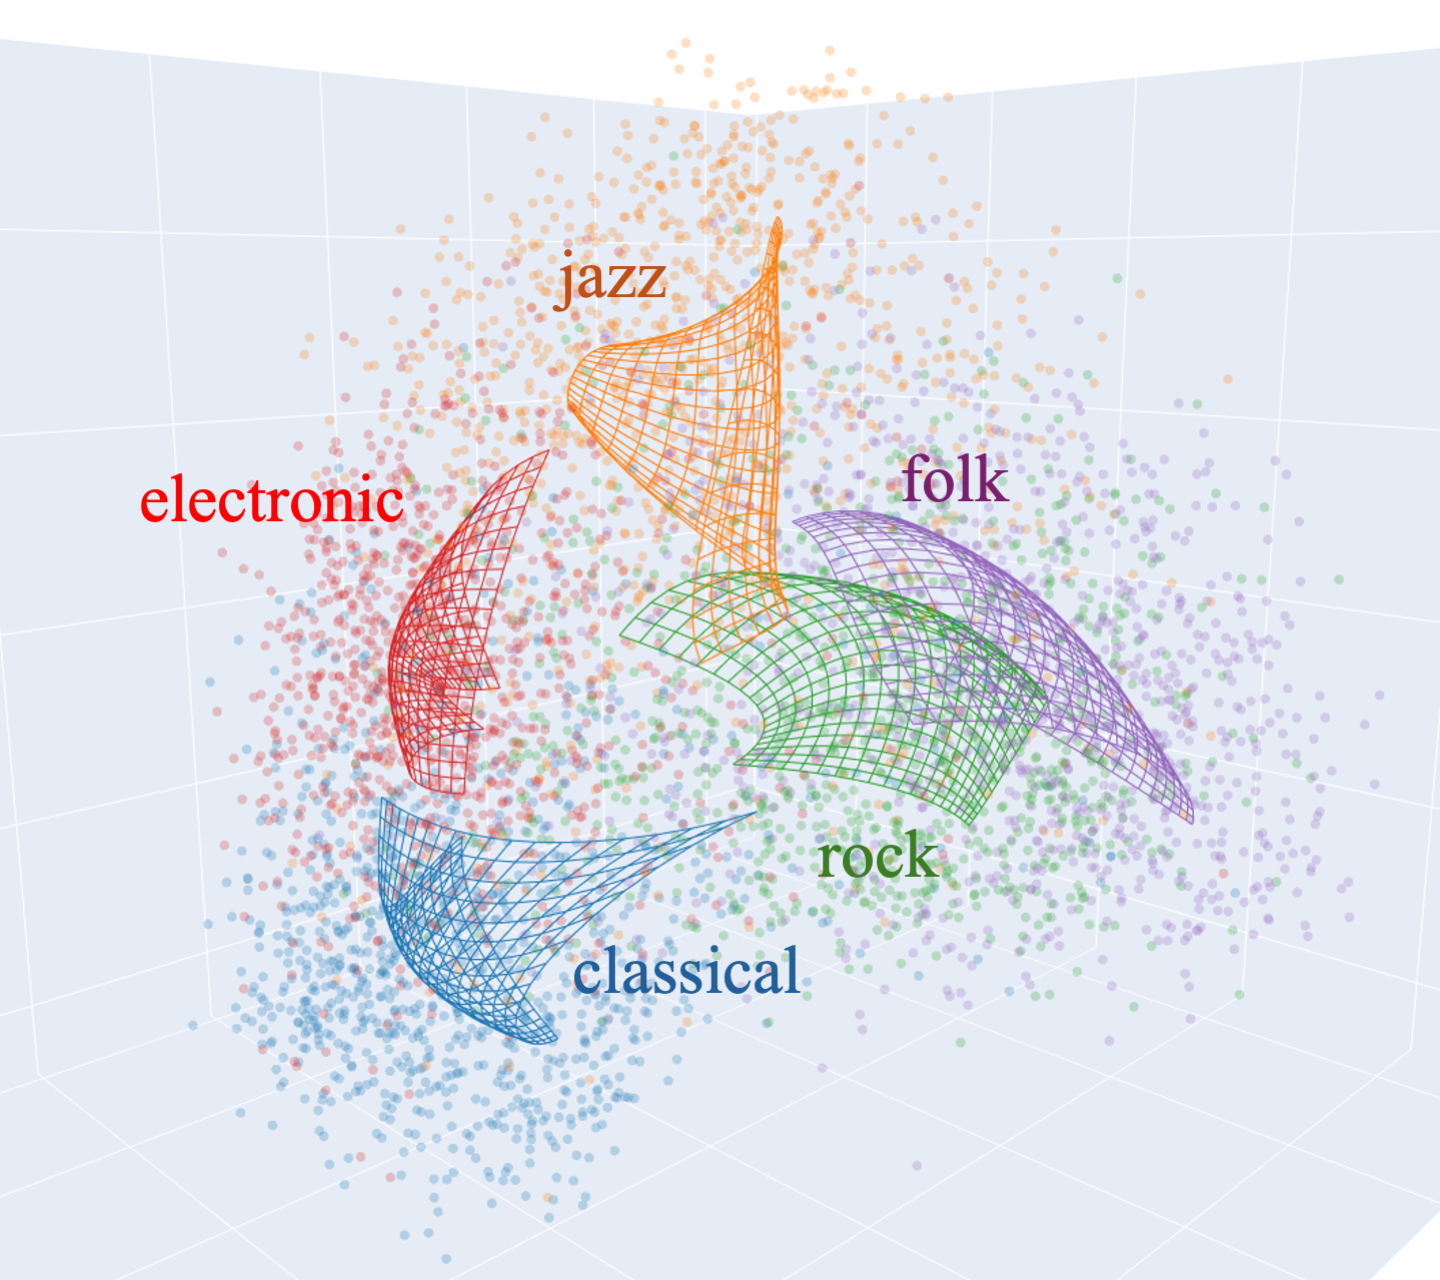
\includegraphics[width=1.0\linewidth]{fig/fig4a.png}
        \caption{Independent manifolds in $\mathcal{X}$.}
    \end{subfigure}
    \hfill
    \begin{subfigure}[t]{0.48\linewidth}
        \centering
        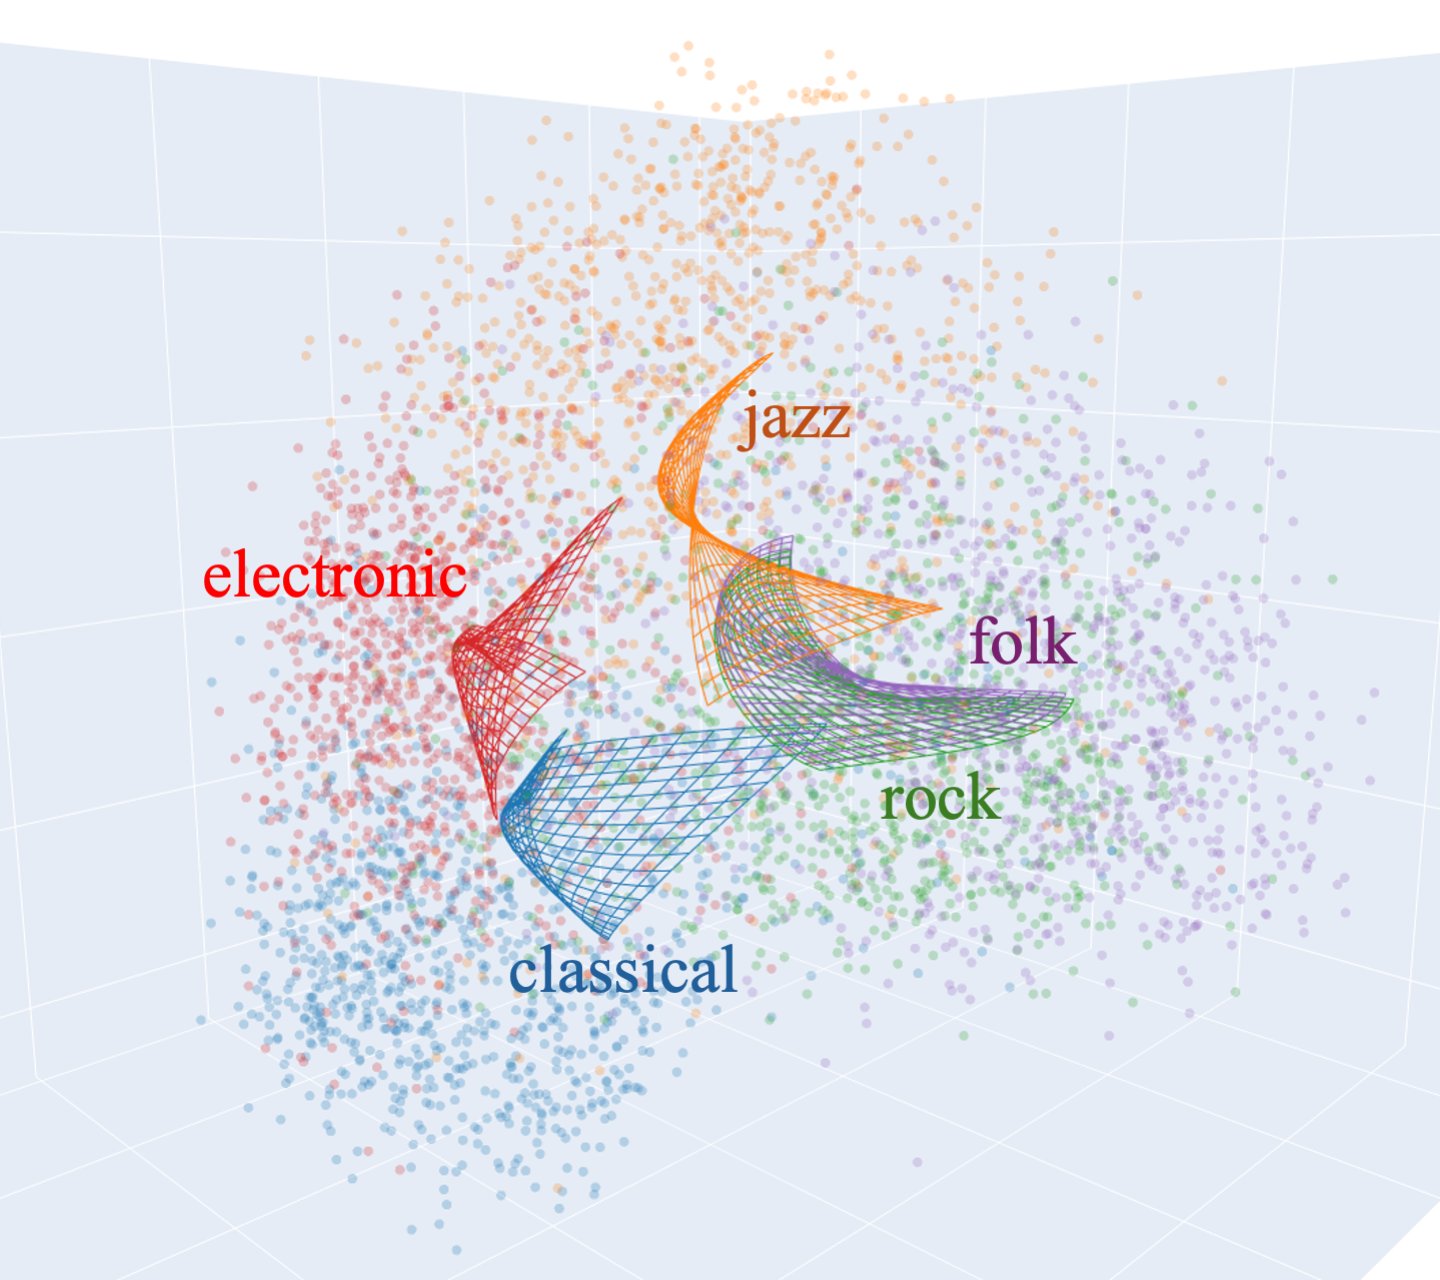
\includegraphics[width=1.0\linewidth]{fig/fig4b.png}
        \caption{The OT-FB in $\mathcal{X}$.}
    \end{subfigure}

    \vspace{2mm}

    \begin{subfigure}[t]{0.38\linewidth}
        \centering
        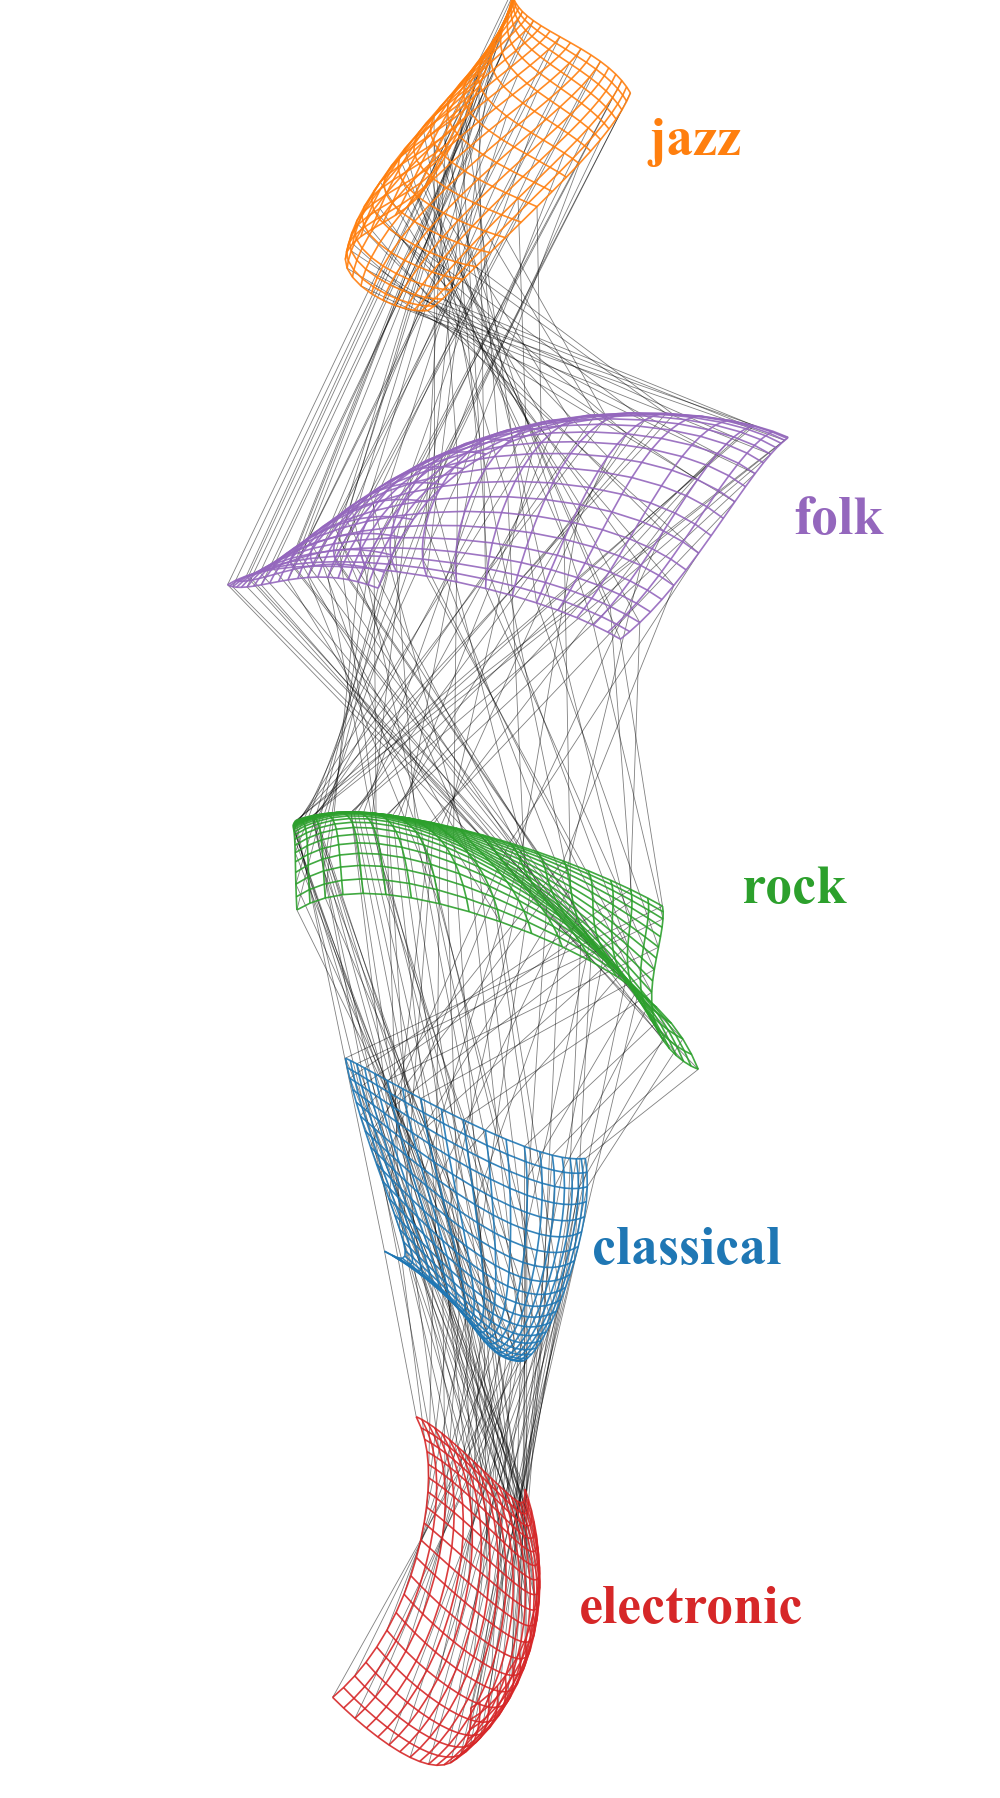
\includegraphics[width=1.0\linewidth]{fig/fig4c.png}
        \caption{Independent manifolds, stacked.}
    \end{subfigure}
    \hfill
    \begin{subfigure}[t]{0.38\linewidth}
        \centering
        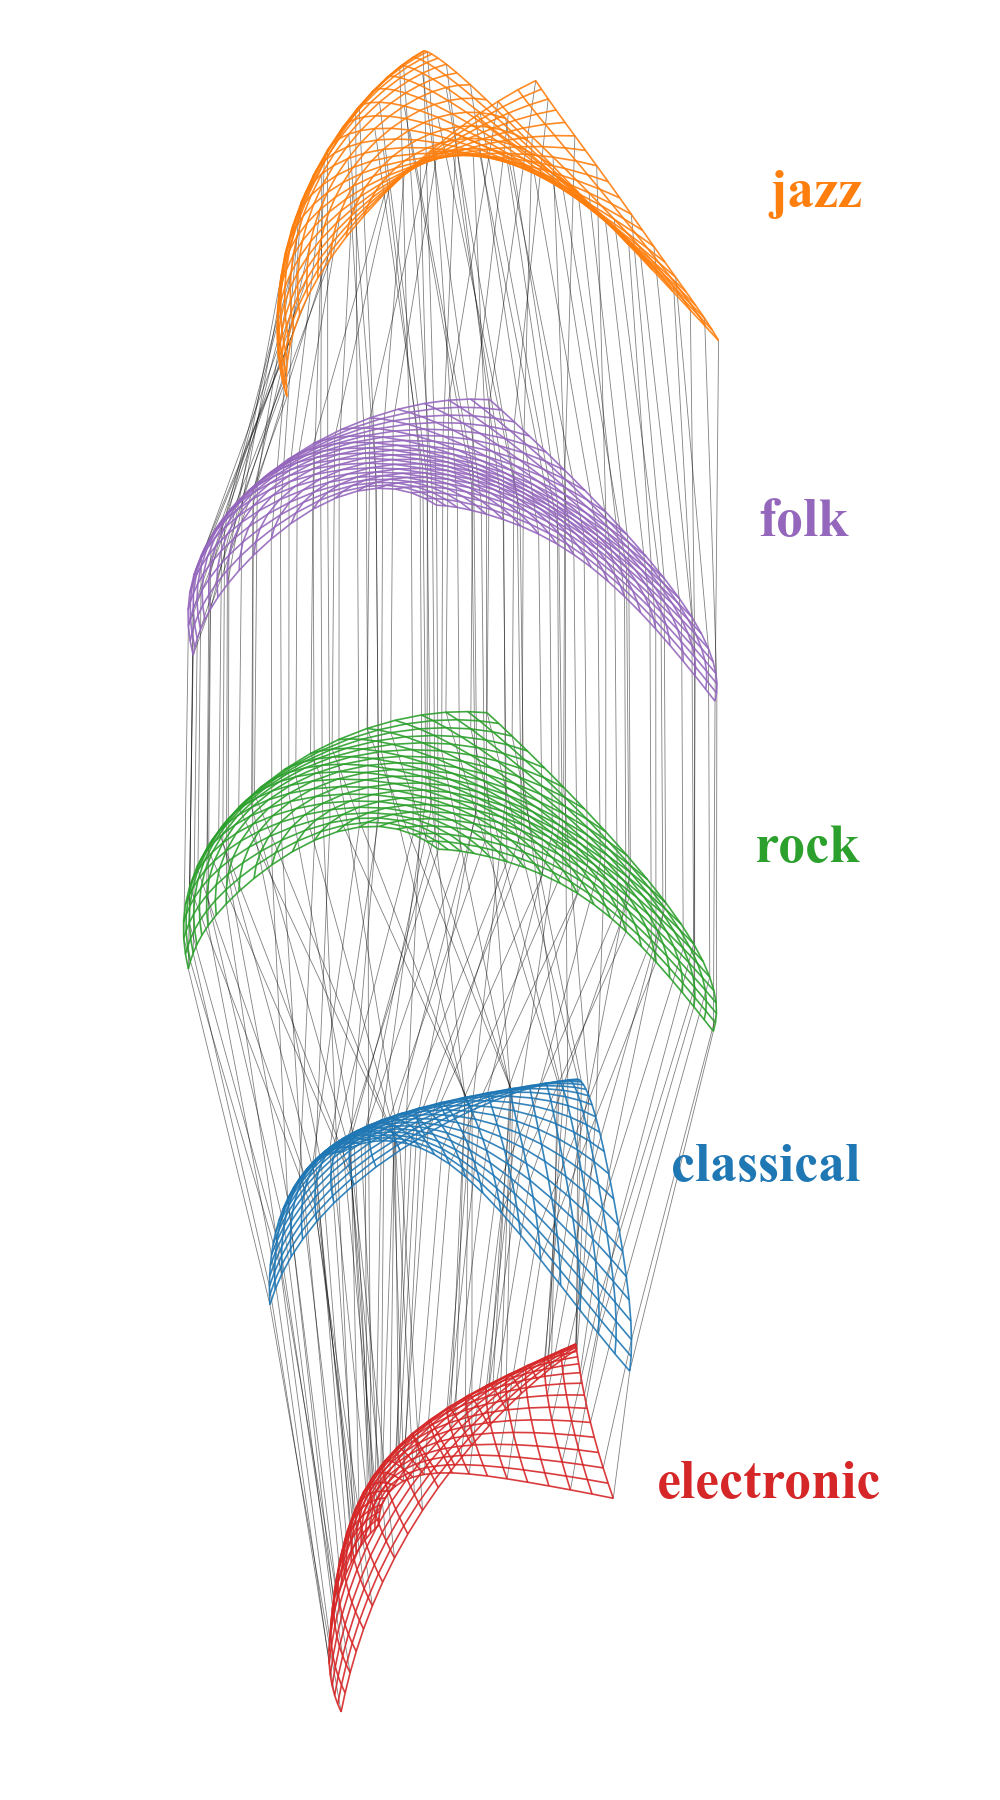
\includegraphics[width=1.0\linewidth]{fig/fig4d.png}
        \caption{The OT-FB, stacked.}
    \end{subfigure}
    \caption{
        \textbf{The five-genre OT-FB learned from MTG-Jamendo.}
        The content data (CLAP embeddings of the audio, first three
        principal components) with the genre manifolds.
        (a) Manifolds fitted independently, one per genre.
        (b) The same five learned jointly as one OT-FB.
        (c, d) The manifolds of (a) and of (b), translated apart and
        stacked as floors; each line joins the same coordinate $v$
        through all five.}
    \label{fig:mtg_otfb}
\end{figure}

%%% Subsection 5.1 %%%
\subsection{A Music Library from Sound and Genre}
\label{subsec:music_library}

\paragraph{Setup.}
The first library is built from MTG-Jamendo~\cite{Bogdanov2019}, an
openly licensed music collection. Five genres---classical, jazz, rock,
electronic, and folk---enter the library, one thousand tracks each, and
every track carries exactly one genre tag. The content data come from
sound alone: each track is embedded by CLAP~\cite{Wu2023}, a joint
audio--text encoder, over excerpts drawn from across it, then averaged,
normalized to unit norm, and reduced by PCA to ten dimensions. These
embeddings and the genre labels are all the modeling uses. The
collection also carries community tags---instruments, moods, and
themes---and they are held out, to be read afterward against the space
the sound itself has built.

\paragraph{The learned bundle.}
Figure~\ref{fig:mtg_otfb} shows the collection modeled by the OT-FB{}.
The five galaxies separate cleanly in the content space
$\mathcal{X}$: sound alone, embedded, already tells the genres apart.
In (a) a manifold is fitted to each galaxy independently; in (b) the
five are learned together as one OT-FB. The fit is much the same, but
the manifolds of (b) are floors of one bundle.

Panels (c) and (d) stack the manifolds apart as floors, each line
joining the same $v$ through all five. In (c) the lines cross and
tangle: every manifold carries a coordinate of its own. In (d) the
same lines descend in order. Five galaxies that lie apart in
$\mathcal{X}$ now share one coordinate system, and each line is a
rabbit hole: five works, one per genre, standing at the same $v$.

Both results satisfy Bias 1: in (c) as in (d), $v$ runs independently
of the genre. Bias 1 alone leaves the floors unaligned. Bias 2 aligns
them, minimizing the total length of the weft.


\begin{figure}[t]
    \centering
    \begin{minipage}[b]{0.47\textwidth}
        \centering
        \begin{subfigure}[b]{0.48\linewidth}
            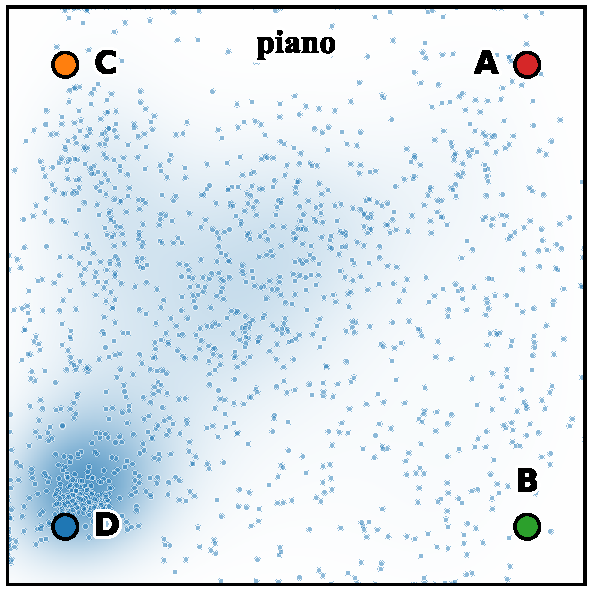
\includegraphics[width=\linewidth]{fig/fig5a.pdf}
            \caption{\textit{piano}}
        \end{subfigure}
        \hfill
        \begin{subfigure}[b]{0.48\linewidth}
            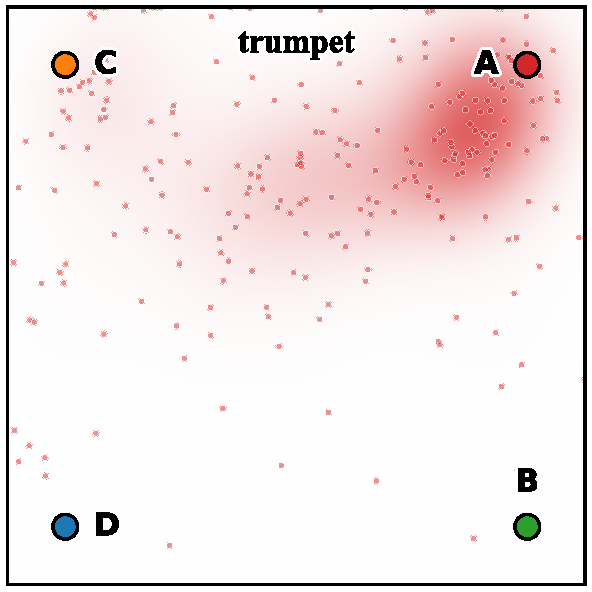
\includegraphics[width=\linewidth]{fig/fig5b.pdf}
            \caption{\textit{trumpet}}
        \end{subfigure}

        \vspace{2mm}

        \begin{subfigure}[b]{0.48\linewidth}
            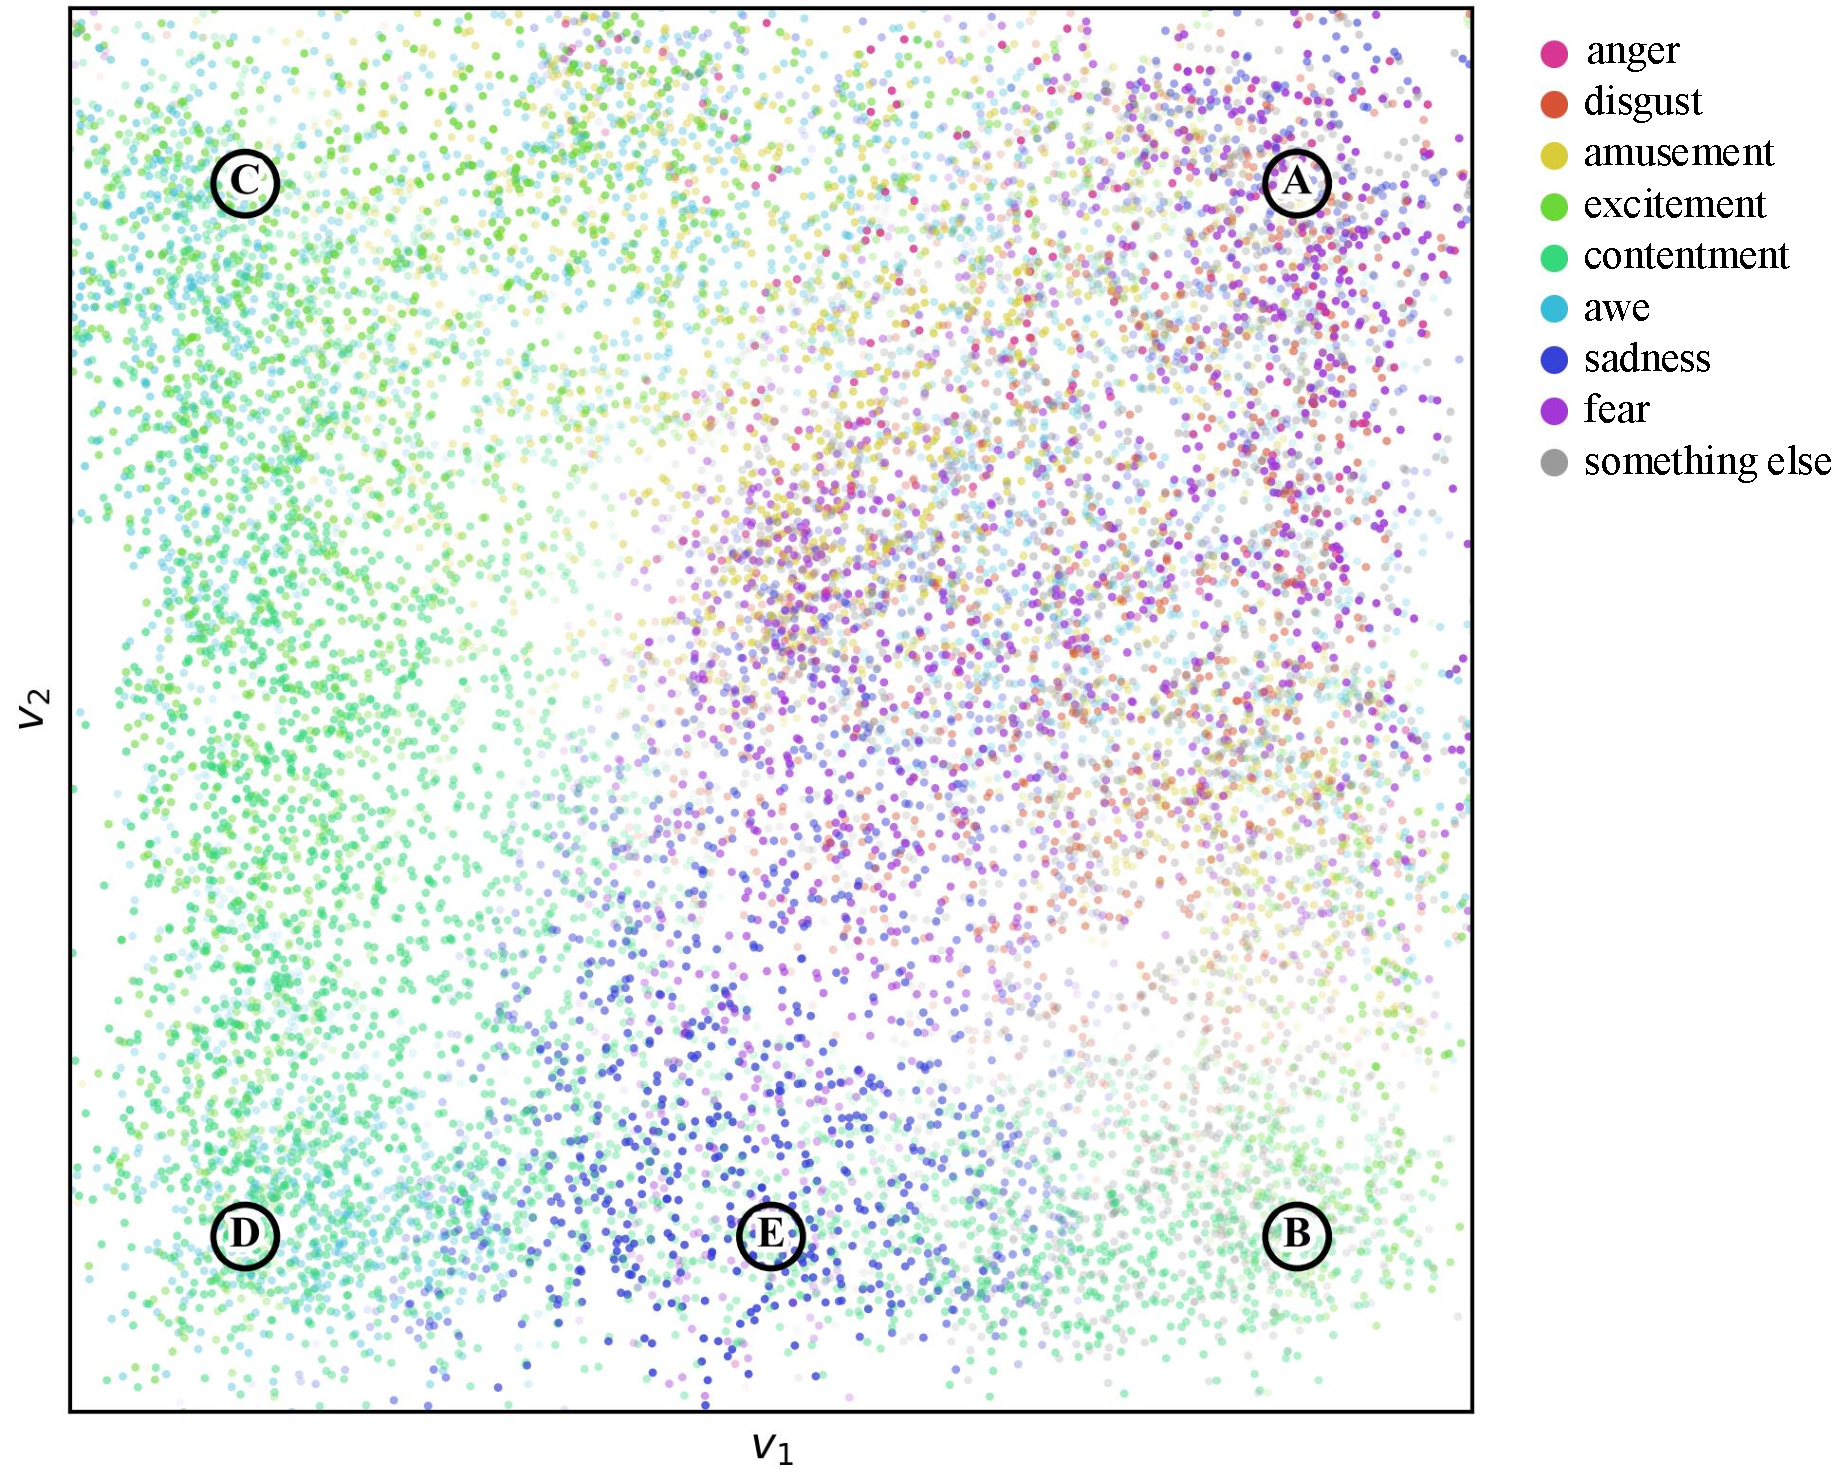
\includegraphics[width=\linewidth]{fig/fig5c.pdf}
            \caption{\textit{acoustic guitar}}
        \end{subfigure}
        \hfill
        \begin{subfigure}[b]{0.48\linewidth}
            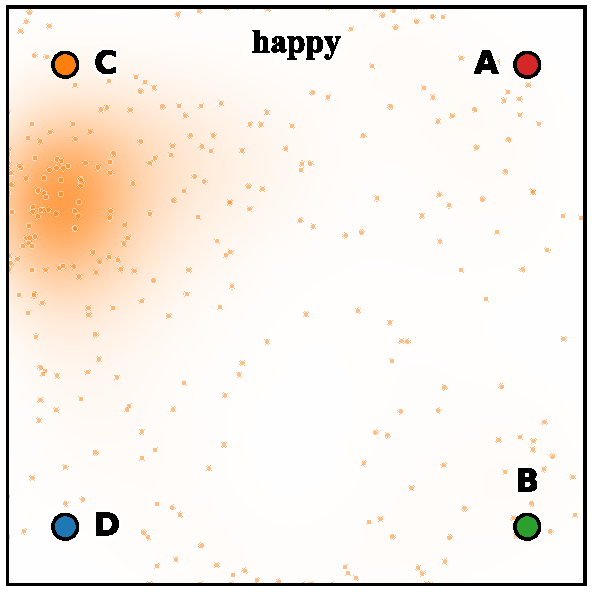
\includegraphics[width=\linewidth]{fig/fig5d.pdf}
            \caption{\textit{happy}}
        \end{subfigure}
    \end{minipage}
    \hfill
    \begin{minipage}[b]{0.51\textwidth}
        \centering
        \begin{subfigure}[b]{\linewidth}
            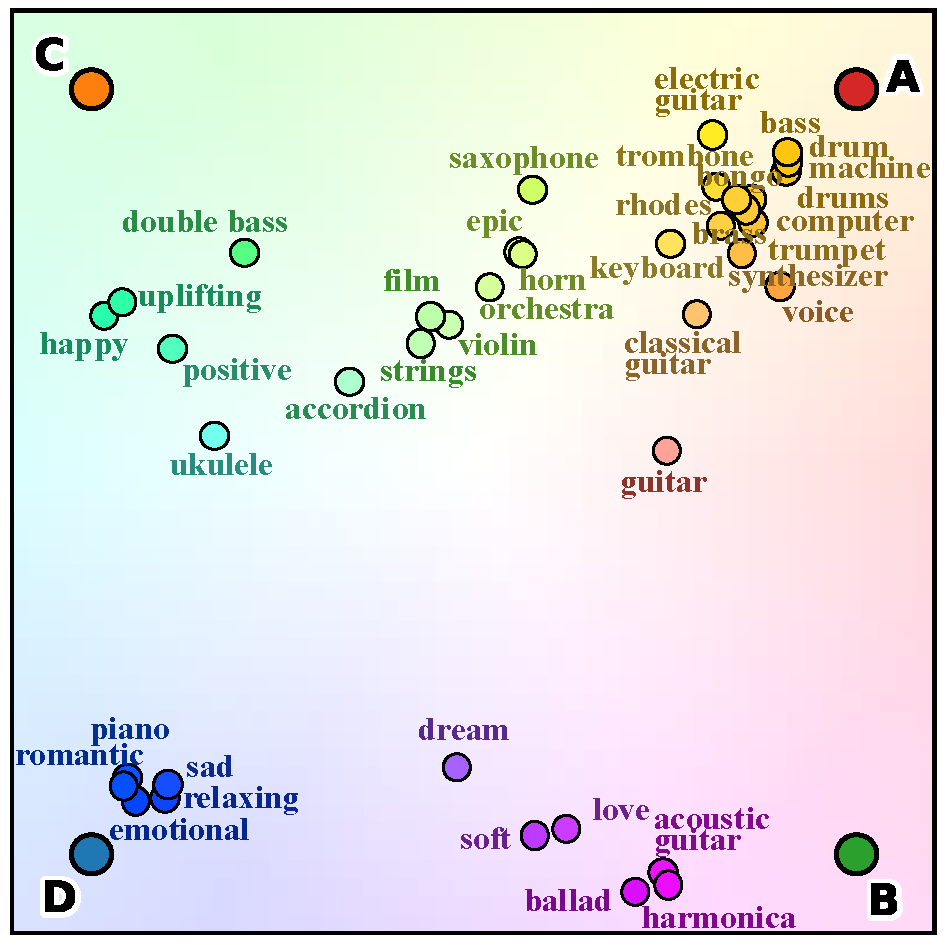
\includegraphics[width=\linewidth]{fig/fig5e.pdf}
            \caption{The landscape of $\mathcal{V}$}
        \end{subfigure}
    \end{minipage}
    \caption{
        \textbf{Reading $\mathcal{V}$ through the tags.}
        (a--d) Where four tags gather: markers show the works
        carrying the tag, and the heatmap is their density
        $p(v \mid \textit{tag})$ by kernel density estimation.
        (e) The top-40 tags by mutual information with $v$, each
        placed at the peak of its density. A peak marks where the
        works carrying the tag concentrate; the layout is not a
        clustering of the tags themselves. Points A--D are those of
        Table~\ref{tab:point_tags}.}
    \label{fig:v_tags}
\end{figure}
\begin{table}[t]
    \centering\small
    \caption{Top 20 tags by mutual information (MI) in units of
        $10^{-3}$ bit.}
    \label{tab:tag_mi}
    \begin{tabular}{@{}clc c clc@{}}
        \cmidrule[\heavyrulewidth]{1-3}
        \cmidrule[\heavyrulewidth]{5-7}
        \textbf{Rank} & \textbf{Tag}    & \textbf{MI} &  &
        \textbf{Rank} & \textbf{Tag}    & \textbf{MI}                               \\
        \cmidrule{1-3} \cmidrule{5-7}
        1             & acoustic guitar & 10.99       &  & 11 & trumpet      & 2.05 \\
        2             & piano           & 8.67        &  & 12 & saxophone    & 2.03 \\
        3             & drums           & 6.63        &  & 13 & computer     & 1.79 \\
        4             & bass            & 4.77        &  & 14 & sad          & 1.51 \\
        5             & voice           & 4.45        &  & 15 & emotional    & 1.45 \\
        6             & electric guitar & 4.11        &  & 16 & drum machine & 1.45 \\
        7             & synthesizer     & 3.60        &  & 17 & love         & 1.44 \\
        8             & ukulele         & 2.59        &  & 18 & violin       & 1.42 \\
        9             & relaxing        & 2.36        &  & 19 & romantic     & 1.41 \\
        10            & happy           & 2.17        &  & 20 & dream        & 1.38 \\
        \cmidrule[\heavyrulewidth]{1-3}
        \cmidrule[\heavyrulewidth]{5-7}
    \end{tabular}
\end{table}


\begin{table}[t]
    \centering\small
    \caption{Representative tags at the four points A--D of
        $\mathcal{V}$: the top five instrument tags and the top five
        mood/theme tags by pointwise mutual information (PMI, in bits,
        in parentheses). Negative PMI is omitted; PMI of at least 1 bit
        is in bold.}
    \label{tab:point_tags}
    \begin{tabular}{@{}c p{0.42\linewidth} p{0.42\linewidth}@{}}
        \toprule
        \textbf{Point} & \textbf{Instrument tags}                               &
        \textbf{Mood/theme tags}                                                  \\
        \midrule
        A              & \textbf{brass (1.18)}, \textbf{bongo (1.12)},
        \textbf{trombone (1.08)}, \textbf{rhodes (1.02)},
        electric guitar (0.96)
                       & fast (0.93), sport (0.84), party (0.78),
        energetic (0.32), powerful (0.30)                                         \\
        \addlinespace
        B              & \textbf{acoustic guitar (1.60)},
        \textbf{harmonica (1.57)}, \textbf{voice (1.21)},
        acousticbassguitar (0.90), percussion (0.82)
                       & \textbf{ballad (1.15)}, \textbf{love (1.04)},
        \textbf{hopeful (1.02)}, mellow (0.98), soft (0.95)                       \\
        \addlinespace
        C              & \textbf{accordion (1.63)}, \textbf{ukulele (1.41)},
        \textbf{double bass (1.29)}, \textbf{trombone (1.15)},
        \textbf{saxophone (1.10)}
                       & \textbf{funny (1.64)}, commercial (0.94), sexy (0.91),
        retro (0.89), summer (0.88)                                               \\
        \addlinespace
        D              & \textbf{piano (1.68)}, pad (0.47)
                       & \textbf{relaxing (1.97)}, \textbf{romantic (1.97)},
        \textbf{sad (1.78)}, \textbf{emotional (1.62)},
        \textbf{calm (1.57)}                                                      \\
        \bottomrule
    \end{tabular}
\end{table}

\paragraph{Reading $\mathcal{V}$ through the tags.} What does the facet-induced
connotation space $\mathcal{V}$ hold? The tags held out of the
modeling---instruments, moods, and themes---give the reading. Each tag defines a
density over $\mathcal{V}$: the distribution $p(v \mid \textit{tag})$ of the
works that carry it. Figure~\ref{fig:v_tags}(a--d) shows four of
them---\textit{piano}, \textit{trumpet}, \textit{acoustic guitar}, and
\textit{happy}. Each peaks at a place of its own, yet the four densities
overlap---connotation runs as a continuous spectrum, not as discrete regions.

Tags differ in how much they tell about $v$. The mutual information
$\mathrm{MI}[v; \textit{tag}]$ measures it: how unevenly the works
carrying the tag fall over $\mathcal{V}$. Table~\ref{tab:tag_mi}
lists the top twenty. Instruments occupy the upper ranks, and moods
follow.

\paragraph{The landscape of $\mathcal{V}$.}
Figure~\ref{fig:v_tags}(e) widens the reading to the top forty tags,
each placed at the peak of its density $p(v \mid \textit{tag})$. Each
tag still spreads around its peak, as (a--d) show; the map marks
where it gathers most.

The landscape divides in two. The upper half is lively: to the right,
drums, bass, electric guitar, and brass---powerful music; to the
left, happy and uplifting. The lower half is quiet: to the right,
acoustic guitar, with love and dream---ballads; to the left, piano,
with emotional, relaxing, sad, and romantic. The two coordinates of
$\mathcal{V}$ carry no names, no more than a principal component
does; yet the landscape they span is legible from end to end.

Table~\ref{tab:point_tags} reads four points more closely: the
corners A--D, each a rabbit hole, seen through the tags concentrated
there. At A the music is fast and energetic, played by brass and
bongo; at B, love ballads on acoustic guitar; at C, funny songs on
accordion and ukulele; at D, piano, relaxing and sad. No single tag
names a point; the tags gathered there do.

\paragraph{What $\mathcal{V}$ represents.}
The tags have read $\mathcal{V}$ as a continuous spectrum. Connotation
itself, though, is known by hearing rather than by words. It lies in
what the works gathered at one point have in common, and no single
word holds it. The tags cannot name it; they let the seeker guess what
a point holds, and a guess is enough to start walking.

What $\mathcal{V}$ holds follows from the facet. Genre was the only
facet, so all else---instruments, moods, themes---was left to
connotation. Which of them, then, does $\mathcal{V}$ carry?

$\mathcal{V}$ carries the two as one. An instrument tends to bring its
own moods---the ring of brass, the cheer of a ukulele, the warmth of
an acoustic guitar. So tags do not settle at points of $\mathcal{V}$.
Each one spreads over a stretch of the spectrum, and the stretches
overlap: \textit{piano} peaks at the lower left, among relaxing and
sad, and reaches the upper right as well, where the music runs
energetic (Figure~\ref{fig:v_tags}(a)). $\mathcal{V}$ is a qualia
spectrum, and its qualia are instrument and mood joined.
\textit{Principal} means this: the two dimensions that account for
that joining with least error (Section~\ref{subsec:content_space}).

A single point of $\mathcal{V}$ does not hold a single kind of music.
The works gathered there are alike in connotation, yet they run from
genre to genre; the space is one, shared by the five. Each point is a
rabbit hole, opening at the same $v$ on every floor. At point A, rock
is energetic music driven by drums; through the hole, on the classical
floor, brass plays with the same force.

Return now to the visitor of Section~\ref{sec:introduction}. The
catalogue told him \textit{trumpet}, and most trumpet music sits at A,
fast and played with force. That is the crowd of trumpeters his search
returned, and almost none of it was what he wanted. What he wanted
lies at D, where trumpets are few, yet present
(Figure~\ref{fig:v_tags}(b)). The name Miles Davis carries him to the
jazz floor and to D upon it, and the hole at D opens onto the
emotional pianos of every other floor. In
Section~\ref{sec:introduction} he made that passage by chance, weeks
later, in a train station. Here it lies under his feet.


\begin{figure}[p]
    \centering
    \begin{subfigure}[b]{0.45\linewidth}
        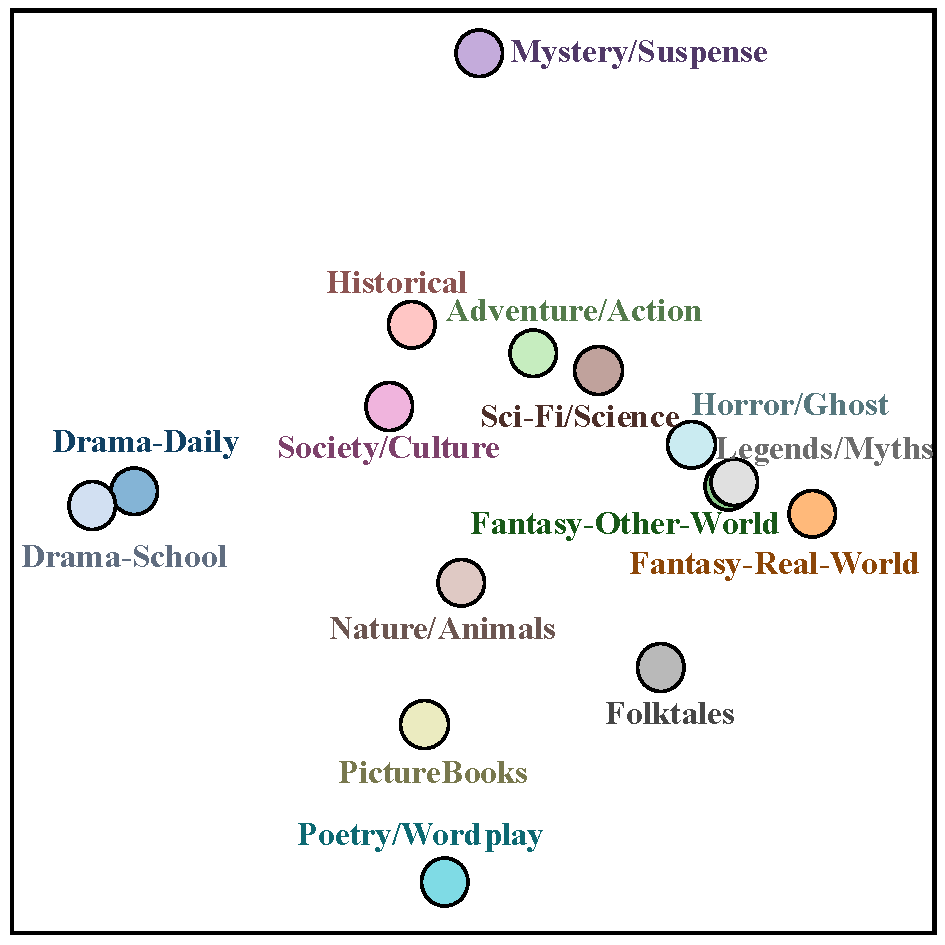
\includegraphics[width=\linewidth]{fig/fig6a.pdf}
        \caption{Spectrum of style/subject}
    \end{subfigure}
    \hfill
    \begin{subfigure}[b]{0.45\linewidth}
        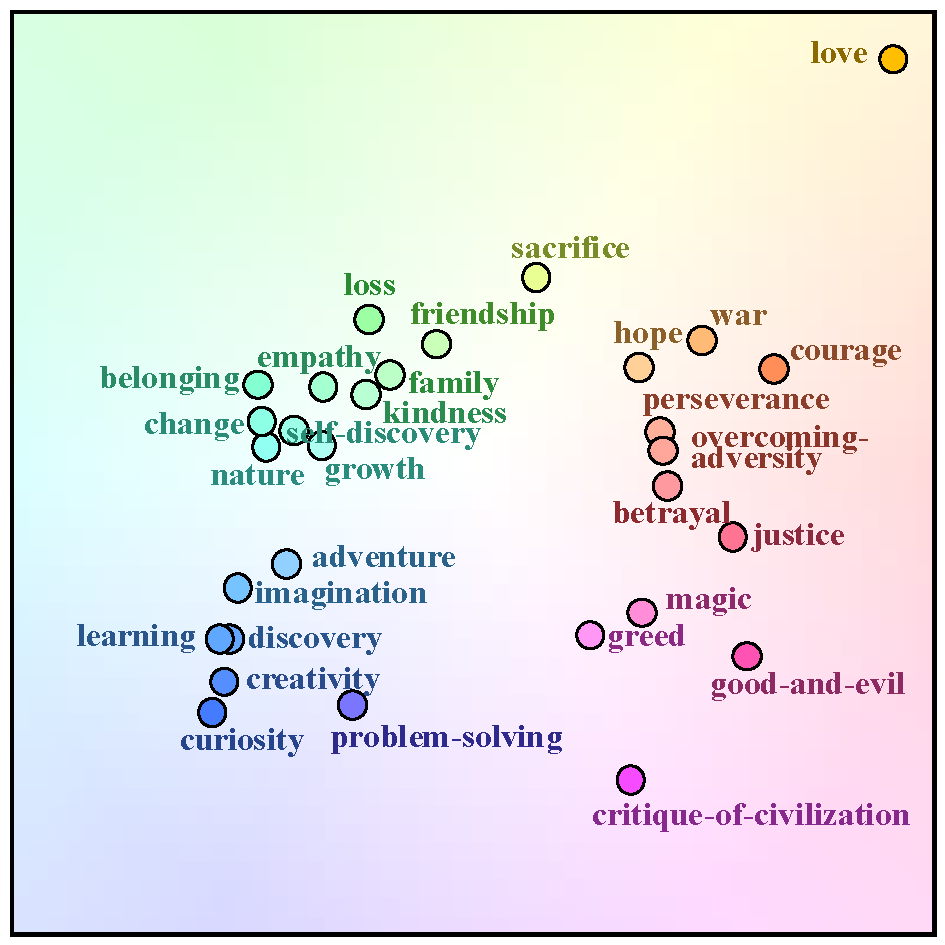
\includegraphics[width=\linewidth]{fig/fig6b.pdf}
        \caption{$\mathcal{U}$ for style/subject}
    \end{subfigure}

    \vspace{2mm}

    \begin{subfigure}[b]{0.42\linewidth}
        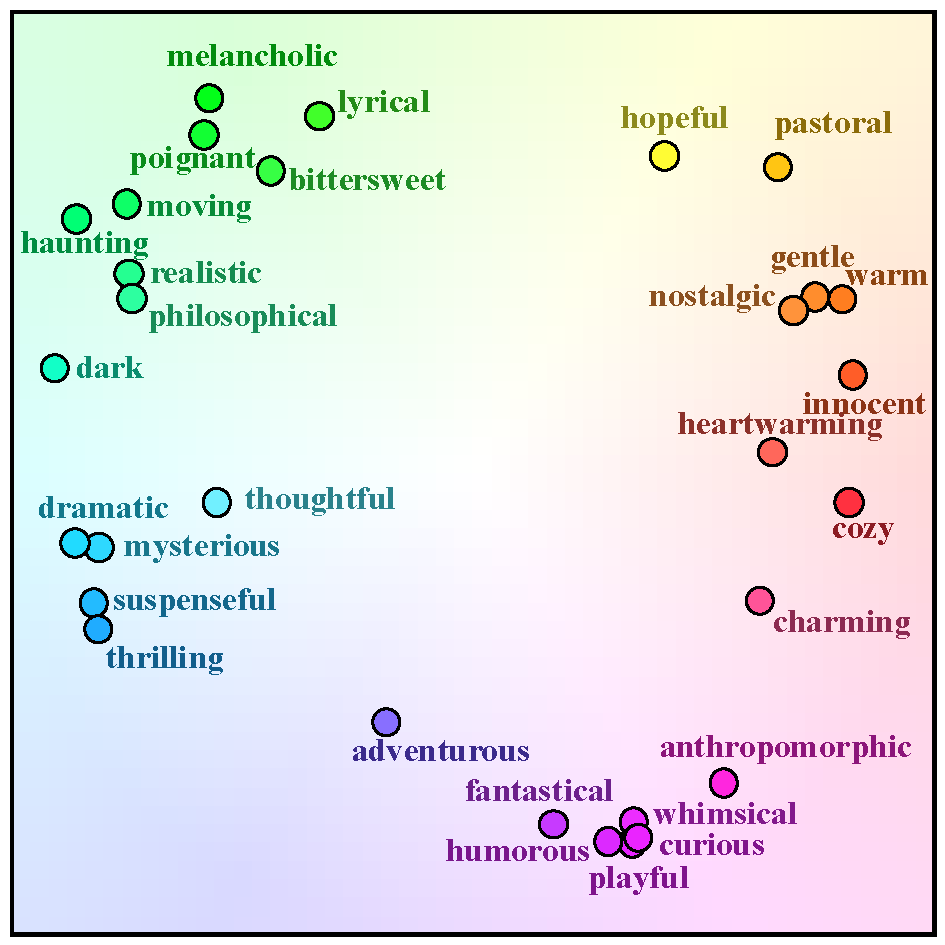
\includegraphics[width=\linewidth]{fig/fig6c.pdf}
        \caption{Words on $\mathcal{V}$}
    \end{subfigure}
    \hfill
    \begin{subfigure}[b]{0.55\linewidth}
        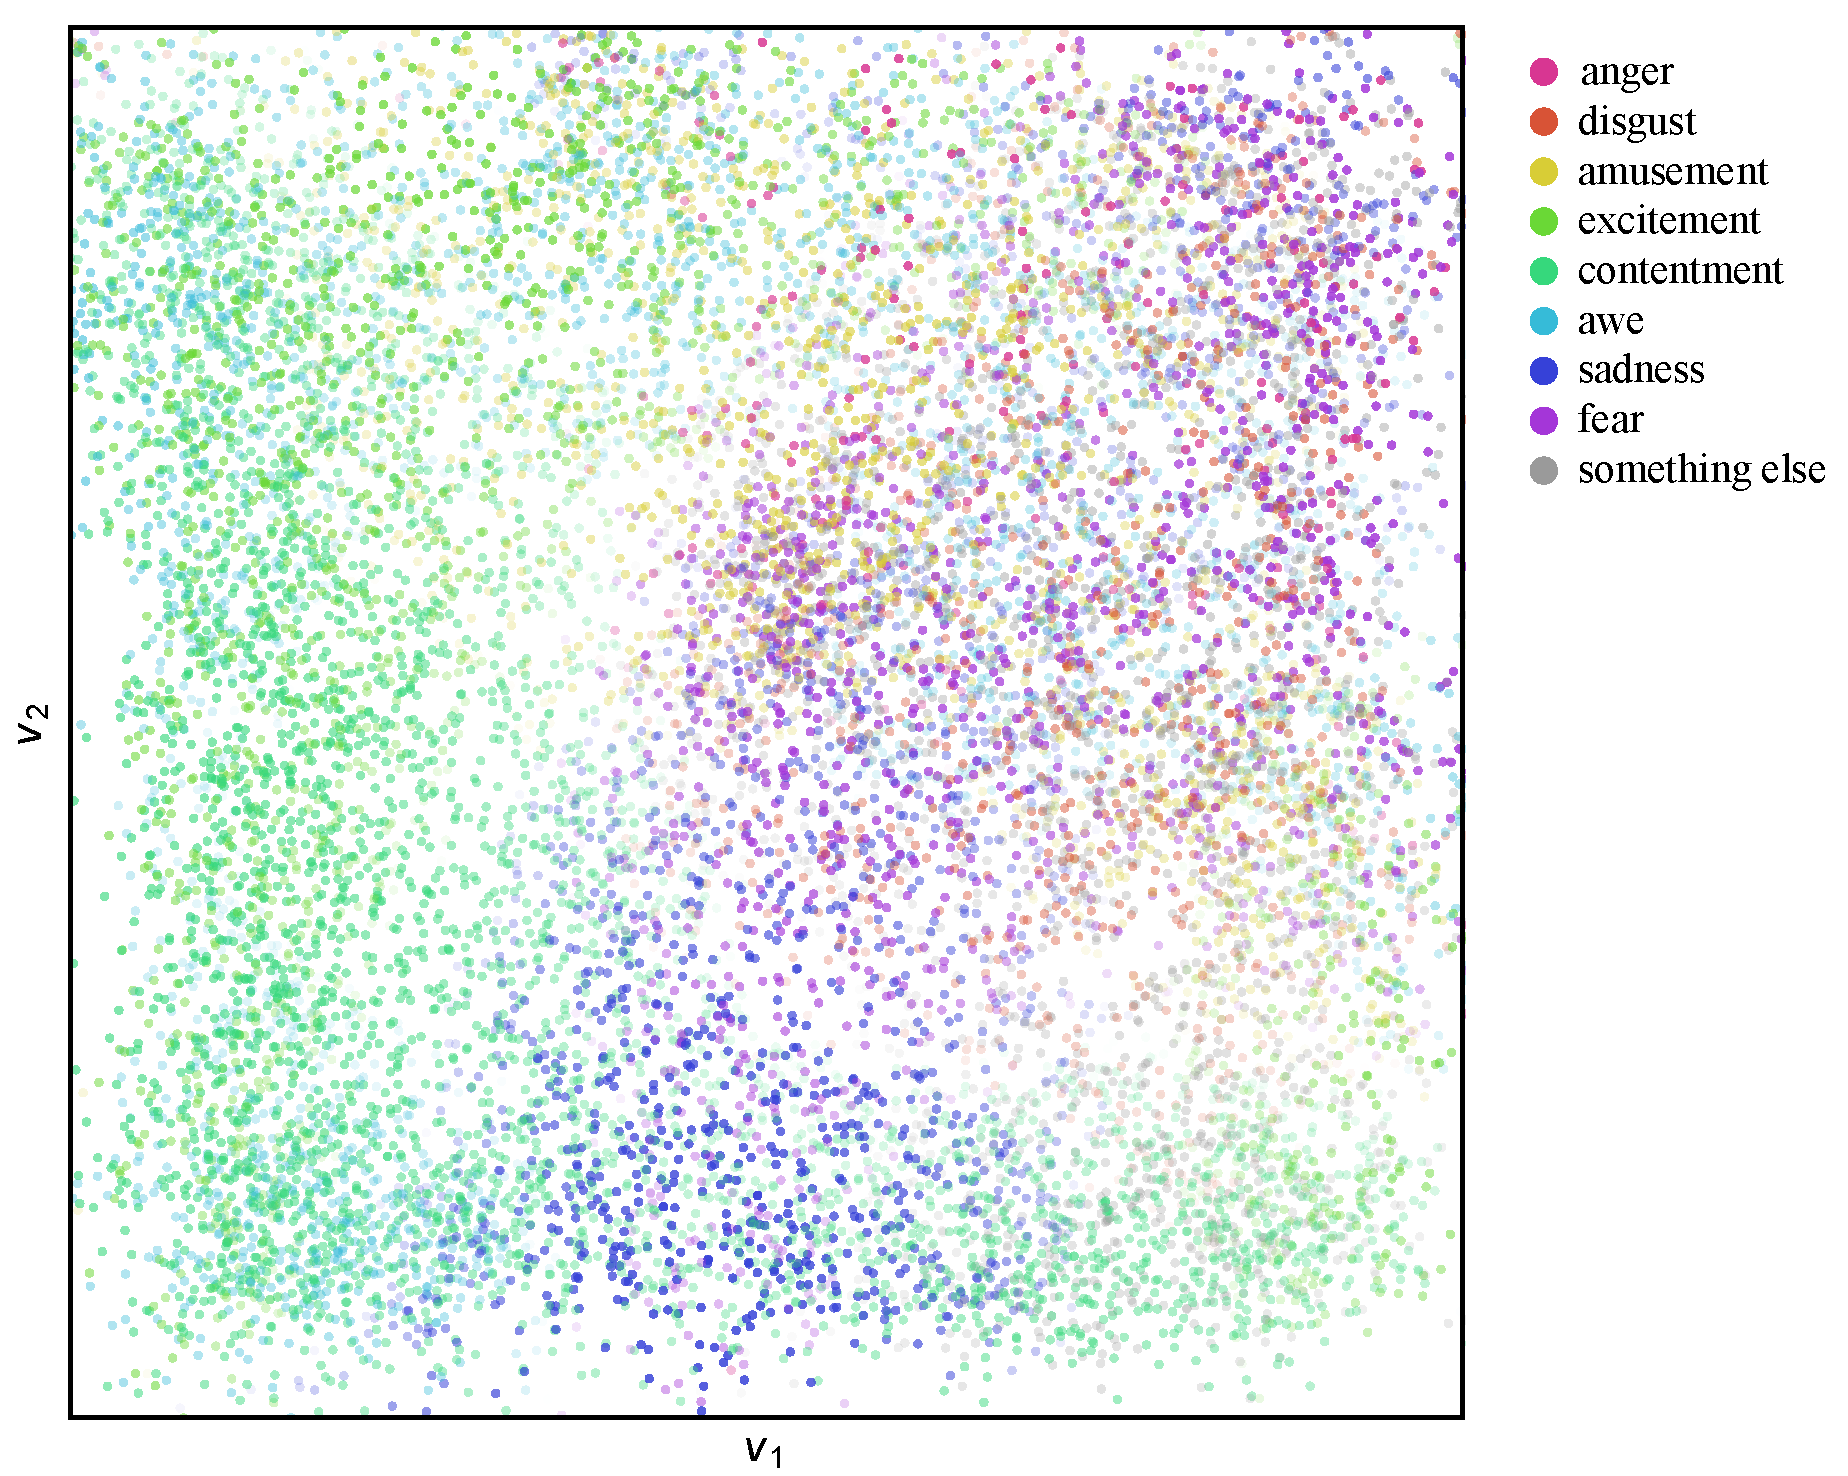
\includegraphics[width=\linewidth]{fig/fig6d.pdf}
        \caption{Emotion on $\mathcal{V}$}
    \end{subfigure}
    \caption{
        \textbf{The twenty-six-floor OT-FB learned from WikiArt.}
        (a) The manifolds in the content space $\mathcal{X}$ (CLIP
        embeddings of the images, first three principal components), one
        per floor.
        (b) The denotation space $\mathcal{U}$. Each marker is one floor,
        its shape the subject: $\triangle$ landscape, $\square$ genre
        painting, $\Diamond$ religious painting, $\bigcirc$ portrait.
        Style runs across, subject runs down.
        (c, d) The connotation space $\mathcal{V}$, read through the
        held-out ArtEmis annotations. Markers sit at the peak of each
        density $p(v \mid \cdot)$: in (c) pairs of emotions, since a
        single emotion peaks in several places while a pair settles in
        one; in (d) words. Larger markers and labels carry higher
        pointwise mutual information with $v$, on each panel's own scale.
        Both panels share one background, the emotion spectrum: the nine
        emotion densities are turned into PPMI, reduced to three axes by
        SVD, and printed as cyan, magenta, and yellow ink on white. Hue
        tells which emotions gather; lightness tells how strongly. White
        marks where no emotion stands out.}
    \label{fig:wikiart}
\end{figure}

%%% Subsection 5.2 %%%
\subsection{A Painting Library from Image, Style, and Subject}

\paragraph{Setup.}
The second library is built from WikiArt, a community-curated
encyclopedia of visual art. Here two facets are given at once: style
and subject. Nine styles, from Baroque to Cubism, meet six subjects
such as landscape and portrait, and every painting carries one name
from each: \textit{Impressionism--landscape}, for instance. All
fifty-four combinations are filled, with up to two hundred paintings
each and nearly nine thousand in all; Figure~\ref{fig:wikiart}(b)
names them. The content data come from the image alone: each painting
is resized whole to 224 by 224, never cropped, and embedded by
CLIP~\citep{Radford2021,Cherti2023}, a joint image--text encoder, then
normalized to unit norm, centered, and reduced by PCA to ten
dimensions. These embeddings and the two labels are all the modeling
uses. The collection also carries ArtEmis~\citep{Achlioptas2021}---%
nine emotions, chosen by a median of six viewers per painting---and
these are held out, as the community tags were.

\paragraph{The learned bundle.}
Figure~\ref{fig:wikiart}(a) shows the fifty-four manifolds in
$\mathcal{X}$, laid out by style and subject. Colour marks $v$: one
colour, one connotation, on every manifold alike. From cell to cell
the surfaces bend and stretch, yet the colours hold their places.
Fifty-four manifolds make one spectrum, as the five genres did.

Read as a library, each style is a floor, and each floor holds six
rooms, one per subject. The rabbit holes join every room to every
other. A visitor may leap to another subject on the same floor, or to
the same subject on another floor, or take both leaps at once---from a
Baroque portrait to a Cubist landscape, in one step. Every leap moves
$u$ and leaves $v$ where it was: the connotation is kept.


\begin{table}[t]
    \centering\small
    \caption{Representative tags at the four points A--D of
        $\mathcal{V}$: the top five annotated words, annotated
        emotions, and painting features by pointwise mutual
        information (PMI, in bits, in parentheses). Negative PMI
        is omitted; PMI of at least 1 bit is in bold. Painting
        features are binarised within each of the 54 classes at
        the 20\% tails, so they are independent of both
        CLIP and the annotations.}
    \label{tab:point_tags_wikiart}
    \begin{tabular}{@{}c p{0.25\linewidth} p{0.24\linewidth} p{0.35\linewidth}@{}}
        \toprule
        \textbf{Point}              & \textbf{Annotated words}                                                                    &
        \textbf{Annotated emotions} & \textbf{Painting features}                                                                                                                                                                                                                                                                                                \\
        \midrule
        A                           & \textbf{black (1.13)}, \textbf{lines (1.10)}, simple (0.87), men (0.84), white (0.78)       & anger (0.67), fear (0.65), disgust (0.26), sadness (0.22), something else (0.19) & \textbf{chroma range (lo) (1.18)}, \textbf{colorfulness (lo) (1.14)}, hue variety (lo) (0.94), chroma (lo) (0.93), lightness (hi) (0.79) \\
        \addlinespace
        B                           & \textbf{flowers (1.08)}, fruit (0.69), red (0.66), colorful (0.62), pink (0.61)             & contentment (0.18), something else (0.13), excitement (0.13), disgust (0.05)     & coarseness (lo) (0.50), colorfulness (hi) (0.50), lightness range (lo) (0.44), chroma (hi) (0.41), hue variety (hi) (0.40)               \\
        \addlinespace
        C                           & \textbf{women (1.11)}, \textbf{people (1.02)}, field (0.99), animals (0.89), vibrant (0.81) & excitement (0.36), awe (0.16), contentment (0.09)                                & self-similarity (hi) (0.94), edge strength (hi) (0.91), brushwork energy (hi) (0.87), anisotropy (lo) (0.85), coarseness (lo) (0.75)     \\
        \addlinespace
        D                           & \textbf{dress (1.23)}, fruit (0.88), street (0.87), skin (0.65), city (0.64)                & contentment (0.27), awe (0.13), excitement (0.07)                                & energy height (hi) (0.59), energy spread (lo) (0.53), lightness range (hi) (0.48), center focus (hi) (0.48), warm (hi) (0.47)            \\
        \bottomrule
    \end{tabular}
\end{table}


\paragraph{The facet map.}
Figure~\ref{fig:wikiart}(b) shows the denotation space $\mathcal{U}$:
the floor-room arrangement of the library. Two facets went in as two
axes, and each axis returned an order.

Style runs in the order of its dates, Baroque to Cubism, though no
date entered the modeling. The spacing is uneven: Expressionism and
Fauvism nearly touch, because their paintings nearly touch in
$\mathcal{X}$.

Subject runs from far to near---cityscape and landscape, then still
life, then genre painting and portrait, and last nude painting. The
view moves from the distant scene to the human body.

Nobody set these orders. Transport places each focus where its works
ask it to stand.

\paragraph{Reading $\mathcal{V}$.}
Figures~\ref{fig:wikiart}(c) and (d) read $\mathcal{V}$ as the tags
read it before. The held-out ArtEmis annotations give two readings:
the emotions viewers reported, and the words they wrote, each placed
at the peak of its density. The background of both panels is the
emotion spectrum itself, so the two readings lie one upon the other.

The reading runs as it did for music. Neither emotions nor words
settle at points; each spreads over a stretch of the spectrum, and the
stretches overlap. And again the two are joined. Where fear gathers,
at the upper left, the words are \textit{dark}, \textit{black},
\textit{lines}, \textit{figure}. Where awe gathers, at the upper
right, they are \textit{mountains}, \textit{hills}, \textit{clouds},
\textit{blue}. Where contentment gathers, below, they are
\textit{flowers}, \textit{dress}, \textit{young}, \textit{peaceful}.
Here too $\mathcal{V}$ is a qualia spectrum, and its qualia are
subject and feeling joined.
%%%%% Section 6. Demonstration with real data %%%%%
\section{Demonstration}\label{sec:demonstration}

Sections~\ref{sec:framework}--\ref{sec:computation} built the library
in concept, in mathematics, and in computation. What remains is to
build one. This section constructs the OT-FB from two actual
collections: a music collection, whose content data come from sound
alone, and a collection of children's books, which carries two kinds
of content data and so receives two bundles of rabbit holes at once.
We first state what the construction asks of the content data, then
build the two libraries in turn.


%%% Subsection 6.1 %%%
\subsection{What the Construction Asks of the Content
    Data}\label{subsec:content_data}

The OT-FB inherits its geometry from the content space. Everything the
construction of Sections~\ref{sec:mathematics}
and~\ref{sec:computation} rests on is measured there: the proximity
assumption (A2) and the transport cost are both stated in the
Euclidean distance of $\mathcal{X}$---the general-purpose inner
product that Section~\ref{sec:framework} asked the content data to
carry. Which works a rabbit hole joins is therefore decided by what
counts as close in $\mathcal{X}$.

The content space must accordingly be \emph{unfolded}: wherever works
are kindred, Euclidean closeness must report it, and wherever works
lie close, kinship must be what brought them there. The demand falls
on neighborhoods, not on the space at large; the space may curve as
it pleases, so long as nearness means kinship. Raw signals do not
satisfy this. Two kindred performances may lie far apart as
waveforms, and two kindred books as word counts, while accidents of
encoding sit side by side; a bundle built on such a space would dig
its holes along those accidents.

Deep embeddings supply spaces of the required kind. Foundation
encoders are trained on large corpora precisely so that semantic
closeness becomes geometric closeness, and their embedding spaces are
unfolded in the sense we need. For sound, we use CLAP~\cite{Wu2023},
a joint audio--text embedding: the music library of
Section~\ref{subsec:music_library} is built from sound alone, with no
words about the works entering the content data.

When the content data are words about the works, an LLM text
embedding plays the same role. The words need not come from a
controlled vocabulary: a ready-made description---an abstract, a
synopsis---serves as it stands, and where none exists, one is
composed from the tags users have freely given---``\textit{this work
carries the following tags: $t_1, t_2, \ldots$}''---and embedded
whole. Nor is a word any longer a label:
\textit{chill} and \textit{relaxed} lie close together in the
embedding, as they do in use. This is, in the end, the visitor's own
method---``\textit{quiet, but with feeling in it}'' was already a
description, offered in whatever words came; an LLM embedding
receives such words and returns a place.

Here one further choice opens: which words are embedded decides what
the bundle carries. Embed the adjectives given to a work, and its
atmosphere enters the content space; embed the nouns, and its themes
do. Section~\ref{subsec:book_library} uses exactly this freedom to
give one collection two kinds of rabbit holes.


%%% Subsection 6.2 %%%
\subsection{A Music Library Built from Sound
    Alone}\label{subsec:music_library}

% MTG-Jamendo (5 genres, exclusive tagging) + LAION-CLAP.
% Content data: audio only; norm normalization + PCA -> X.
% Genre only is given for training; mood/theme tags are held out
% and meet V afterward.
% TODO: 実験結果待ち。パラグラフ設計は結果より先に行う。


%%% Subsection 6.3 %%%
\subsection{A Book Library with Two Kinds of Rabbit
    Holes}\label{subsec:book_library}

% 400 children's books; adjective tags (atmosphere) and noun tags
% (themes) -> two LLM text embeddings -> two bundles:
% (u, v_atm, v_theme). Tag-to-description recipe
% ("This item has the following tags: ...") を setup に一文で再掲。
% Ver.2 (paper202605) の結果を移植して書き直す。

%%%%% Section 7. Discussion %%%%%
% 2026-08-03 全面差し替え。旧稿(Ver.2 コピー)は破棄。
% §7.1 のみ執筆済み。残る subsections(図書館への含意/予期される反論/
% 表現とインターフェース 等)は未執筆(instructions.md §4 参照)。
% 2026-08-08: 応用システム/rating-as-content/record への追記(客観性・普遍性)の
% 3 subsections を末尾に追加(見出し仮)。内容メモ(コメント)+暫定散文(Claude 叩き台)。
\section{Discussion}\label{sec:discussion}

%%% Subsection 7.1 Where Connotation Lives %%%%%
% 見出しは仮(2026-08-03)
\subsection{Where Connotation Lives}\label{subsec:where_connotation}

% --- P1: sec2 の record の非対称 → 単位の非対称へ ---
Section~\ref{subsec:naming} located the difference between the two
kinds of attribute at the record: denotation arrives with it,
connotation is written in no field. The bundle locates the
difference more deeply---at the unit. A name is attached to one
work at a time; what the OT-FB expresses is not a property of one
work at all.

% --- P2: 三段の認識論(pairwise で不可視 → ドメイン内で構造 → ドメイン間で independence)---
Consider a collection of two works. Between them there is a
distance, and nothing more---nothing to say how much of it is
genre and how much runs across genre. Connotation is not hidden
in such a world; it has nowhere to exist. Within a genre, among
many works, it takes shape: each work shares some connotations
with some works and not with others, and this web of shared and
unshared gives every work a relative position among its own kind.
And it is only across genres that the last question can be put:
which part of this shape is independent of the genre itself?
Where the ensembles correspond as wholes, galaxy laid onto
galaxy, what the correspondence preserves is shared across
domains---and being shared across domains is what
\emph{independent of denotation} means. Such a whole-to-whole
correspondence is what transport computes, and what no pairwise
comparison can.

% --- P3: だから single word にならない(語彙ではなく単位の不一致)---
This is why connotation was never going to be carried whole by a
name. A name attaches to the individual work; connotation, as the
bundle draws it, lives in the relations among domains. The
consistent failure of connotative naming that
Section~\ref{subsec:naming} recorded is, on this reading, not a
poverty of vocabulary but a mismatch of unit---and a coordinate
does not enrich the vocabulary; it changes the unit.

% --- P4: principal connotation =道しるべ(切り捨ては設計判断)---
Nor does the bundle keep every connotation. The principal
connotation analysis of Section~\ref{subsec:bundle_reach} retains
what is independent of denotation, present in the content data, and
principal among what remains; whatever depends on the genre is
left with the genre. This is a design decision, not a shortfall.
An axis whose meaning shifted from floor to floor could not guide
a leap; what can serve the explorer as a signpost is exactly what
keeps its meaning on every floor. The rabbit hole is dependable
for the same reason it is partial.

%%% Subsection 7.2(仮)Reading Connotation from Language %%%%%
% 2026-08-11 新設。内容メモ(コメント)+暫定散文(Claude 叩き台)。見出し・位置仮。
% 位置の根拠: §7.1 が「connotation はどこに宿るか」(関係・単位)を言い、本節が
% 「その関係をどのデータから、誰が読むのか」を引き受け、§7.x(From Representation
% to Systems)の query by description へ渡す。したがって §7.1 の直後・§7.x の直前。
%
% --- 内容メモ(2026-08-11 せんせーとの対話で確定)---
% (0) 本節が回収する伏線: §2.2 の `An information system cannot rely on such
%     background implicitly`(shared background = language, culture, embodied
%     experience。Clark1996 / Langacker2008 / Hjorland1995400)。
%     回答は「背景に頼らない」ではなく「背景の痕跡から読む読み手をシステムが所有する」。
% (1) **成立条件としての generic feature vector**(せんせー 2026-08-11)。
%     かつて feature vector は用途ごとに設計するものだった——何を特徴とするかを
%     設計者が事前に決める。それは名前を事前に選ぶことであり、§2.2 の Osgood の
%     `the scales themselves must still be chosen in advance` と同じ構造。
%     すなわち denotative manner で connotation を作ることと五十歩百歩だった。
%     generic embedding は用途に先立って存在し、設計者は次元の意味を選ばない。
%     だから初めて「データが軸を決める」余地が生じた。**これが本手法の背景**。
% (2) LLM は言語化装置ではなく**読者**。タグ列は言語(denotative なラベル列)だが、
%     connotation は列そのものではなく「列を読んだときに立ち上がるもの」に宿る。
%     ベクトルはその読みの残したもの。
% (3) 主張の限定——存在論ではなく操作論(せんせー 2026-08-11 確定)。
%     ×「LLM は embodiment を備える」/ ×「meaning を再現する」
%     ○「間接的かつ部分的ではあれ、connotative な情報が内部のベクトル表現から
%        引き出せる」。検証可能な主張の形に置き直すことで、決着しない存在論を通らない。
%     「部分的」は新たな譲歩ではなく §4.3 principal への三つの限定と同じもの
%     (→ §7.1 末尾 `dependable for the same reason it is partial` と韻を踏む)。
% (4) seeker 側と work 側は同じ読み手。LLM は現にプロンプトから connotation を
%     読む(読者自身の日常経験)。同じ読み手が works の側も読むから、query と work が
%     同じ空間に落ちる——§7.x の query by description の**機構がここで与えられる**
%     (現行の暫定散文 `lands somewhere in the connotation space` は機構を語っていない)。
%     ただし「現に読み解いている」は振る舞いの証拠であって表現の幾何の証拠ではない。
%     ゆえに順序は「幾何を測った研究(P3)→ 日常経験(P4)」とし、逆にしない。
% (5) 反対側への態度: form から meaning へ到達するとは主張しない。得るのは works の
%     **配置**であり、座標は何も名指さない(sec3)。BenderKoller2020 / Bisk2020 の
%     否定命題を認めたまま本論文の主張は無傷で通る。敬意を持って引く。
%
%%% TODO 引用(2026-08-11 Web 検索で実在確認済み。bibkey は仮・**ページ未確認**——
%%% ref.bib 追加時に一次ソースで巻号ページを検証すること。命名は既存則(著者+年+開始頁)に揃える):
%%%  (i)  Louwerse & Zwaan (2009) "Language Encodes Geographical Information,"
%%%       Cognitive Science 33(1). 都市名の共起統計のみから緯度経度が復元できる。
%%%       「言語には誰も書かなかったものが刻まれている」の最も直截な実証。→ 主柱1
%%%  (ii) Louwerse (2011) "Symbol Interdependency in Symbolic and Embodied Cognition,"
%%%       Topics in Cognitive Science 3(2). symbol interdependency hypothesis——
%%%       言語のシンボル体系は身体的・知覚的経験の痕跡を符号化している。
%%%       せんせーの「間接的に身体性を備えている」に認知科学側で付いている名前。→ 主柱2
%%%       (関連: Louwerse (2018) "Knowing the Meaning of a Word by the Linguistic
%%%        and Perceptual Company It Keeps," Topics in Cognitive Science 10(3).)
%%% (iii) Grand, Blank, Pereira & Fedorenko (2022) "Semantic projection recovers rich
%%%       human knowledge of multiple object features from word embeddings,"
%%%       Nature Human Behaviour 6(7). word embedding から**軸への射影**で人間の
%%%       特徴知識(size/danger/intelligence 等)を復元。§4.3 principal connotation
%%%       analysis と操作が同型。掲載誌の格も JDoc 読者に効く。→ 主柱3(最重要)
%%%  (iv) Marjieh et al. (2024) "Large language models predict human sensory judgments
%%%       across six modalities," Scientific Reports 14(arXiv:2302.01308). 補強。
%%%  (v)  Abdou et al. (2021) "Can Language Models Encode Perceptual Structure Without
%%%       Grounding? A Case Study in Color," CoNLL. 色の知覚構造。補強。
%%%  (vi) 反対側(敬意を持って引く): Bender & Koller (2020) "Climbing towards NLU,"
%%%       ACL / Bisk et al. (2020) "Experience Grounds Language," EMNLP.
%%% 既に ref.bib にあり本節で再出させうるもの: Clark1996, Langacker2008,
%%% Hjorland1995400(§2.2 で既出), Deerwester(LSA, 未使用)。
\subsection{Reading Connotation from Language}\label{subsec:reading_connotation}

% --- 以下、メモを実現する暫定散文(2026-08-11、Claude 叩き台)---
% --- P1: 成立条件(generic feature vector)= 本手法の背景 ---
The method has a precondition, and it is recent. Feature vectors were
once built for a purpose: whoever built them decided beforehand what
would count as a feature, and that decision was a choice of names.
Osgood's scales had to be settled before the rating began
(Section~\ref{subsec:naming}); a hand-built feature set makes the same
choice, in numbers rather than in words, and arrives at connotation by
denotative means. Generic embeddings come before any purpose. Nobody
has decided, for this collection, what the dimensions are to mean---
nothing in them has been named. Only under that condition is there room
left for the data to decide where the axes lie.

% --- P2: LLM は読者である(§2.2 の伏線回収)---
What such an embedding reads is language, and yet connotation is not in
the language it reads. A list of tags---genre, mood, era,
instrument---is a string of denotative labels; read them together, and
something rises that no one of them holds. This is the work the language
model is put to. It is not asked to name, but to read, and the vector is
what its reading leaves behind. Section~\ref{subsec:naming} observed
that between people connotation travels unnamed, on a shared background
of language, culture, and embodied
experience~\cite{Clark1996,Langacker2008,Hjorland1995400}, and that a
system cannot lean on that background implicitly. It need not. It can
hold a reader who has come by that background at second hand.

% --- P3: 主張の限定 + 認知科学の足場(測られていること)---
How much of the background such a reader has is a fair question, and the
claim we make is narrow. Not that a language model has embodied
experience; not that it recovers meaning. Only that connotative
information is present in its internal vectors and can be drawn out of
them---indirectly, and in part. That much has been measured rather than
assumed. Language carries the trace of perceptual experience: from the
co-occurrence statistics of city names alone, latitude and longitude can
be recovered~\cite{LouwerseZwaan2009}---a regularity Louwerse names
symbol interdependency~\cite{Louwerse2011}. Human judgments of object
features are recovered from word embeddings by projection onto an
axis~\cite{Grand2022}, which is the operation of
Section~\ref{subsec:bundle_reach} performed on other data. Language
models predict human sensory judgments across
modalities~\cite{Marjieh2024}, the structure of color among
them~\cite{Abdou2021}. Whether form can suffice for meaning remains
contested~\cite{BenderKoller2020,Bisk2020}, and this construction does
not need it to: what it claims to obtain is an arrangement of works, not
their meaning, and the coordinate marks a place while naming nothing
(Section~\ref{sec:framework}).

% --- P4: 一人の読み手が両側を読む → §7.x の query by description へ渡す ---
One reader serves both sides. A language model reads connotation from a
prompt as readily as from a list of tags---which is the ordinary
experience of anyone who has used one. The groping description of
Section~\ref{subsec:representation_to_systems}, then, and the works it
gropes for are read by the same reader, and fall into the same space.
The seeker's few words and the collection's many are commensurable
because of who reads them.


%%% Subsection 7.x(仮)From Representation to Systems %%%%%
% 2026-08-08 下書き。内容メモ(コメント)+暫定散文(Claude 叩き台)。
% 見出し・位置・順序はすべて仮。既定の残り subsections
% (図書館への含意/予期される反論/表現とインターフェース)との統合・分割は
% 執筆時に判断する。とくに「表現とインターフェース」(v9 §9)とは対句の関係:
% v9 §9 =「interface ではなく representation を」(貢献の位置づけ)、
% 本節=「representation が得られたいま、その上に interfaces は増殖する」(展望)。
\subsection{From Representation to Systems}\label{subsec:representation_to_systems}

% --- 内容メモ: disentangled representation からどんな情報システムが作れるか ---
% (1) ウサギ穴付き図書館: representation をそのまま探索空間にする。
%     従来型の denotative なシステムにウサギ穴を「追加」する形式も可能だし、
%     denotative space ごと探索可能な空間にすることもできる。
% (2) 関連作品による connotation 検索: 該当しそうな works を利用者が例示して
%     (例: Miles Davis の "Kind of Blue")、「connotation が共通する他の作品」を
%     検索・探索する。
% (3) Fuzzy description 検索: 「静かで、色彩的で、しかもそれらが溶け合ったような……」
%     という自然言語的表現や、関連しそうな単語列から connotation 検索・探索する。
% (4) 典型的タグによるスライダー検索(2026-08-08 追加): connotative axis と
%     相互情報量の高いタグへのマッチ度をスライダー(0/1 の二値も可)で指定して
%     検索・探索する。これを備えると Book House(アイコン入力)も取り込める。

% --- 以下、メモを実現する暫定散文(2026-08-08、Claude 叩き台)---
Section~\ref{sec:introduction} argued that representation must come
first, because no interface can surface what the space beneath it
does not encode. The converse deserves a word: once the space
exists, interfaces multiply. The most direct is the library of
Section~\ref{sec:framework} itself---rabbit holes added to an
otherwise conventional denotative catalog, or a space in which the
floors themselves are open to walking. A second is query by works:
a seeker offers what can be named---\textit{Kind of Blue}---and asks
for works that share its connotation, wherever their genres lie. A
third is query by description: a groping, natural-language
gesture---``quiet, and full of color, and the colors run into one
another''---lands somewhere in the connotation space, and the
neighborhood does the rest. A fourth returns an earlier idea to
service. Tags that share high mutual information with a connotative
axis can stand for that axis, and a seeker can set, slider by
slider, how much of each they want---continuously, or simply on and
off. This is recognizably the Book House~\cite{Pejtersen1983230},
its icons refounded: what once lived in the session can now read
from a space that outlives it. Different entrances, one space; what
varies is only how the seeker points.

%%% Subsection 7.y(仮)Rating Data as Content Data %%%%%
% 2026-08-08 下書き。内容メモ(コメント)+暫定散文(Claude 叩き台)。
\subsection{Rating Data as Content Data}\label{subsec:rating_as_content}

% --- 内容メモ: collaborative filtering の user-item rating data を content data と
%     みなして disentangled representation を作る ---
% * ウサギ穴(disentangle された axis)との相互情報量が高い curator には、
%   その名前をウサギ穴に付けることができる——「○○さんのウサギ穴」。
%   curator 全員ではなく、axis との関連度(相互情報量)の高さで基準となる
%   curator を見つける、という選び方。
% * ユーザー側から見れば、「自分の中にある何か」と resonate する curator を
%   探索的に見つけられる、という読み替えにもなる。
% * "curator" という語が適切かどうかは要検討(暫定散文では curator を仮使用)。
% * 既決との接続(2026-08-04 整理): rating data は content data と同等に扱える。
%   recsys との本質差は data source ではなく「ユーザーをモデル化するか」——
%   ここでは同じ rating data から works をモデル化する。§2.3 の書き方と揃える。

% --- 以下、メモを実現する暫定散文(2026-08-08、Claude 叩き台)---
Nothing in the construction requires that the content data be sound
or text. A work is described by those who attend to it as well as
by what it contains: the ratings a work gathers across many
listeners are themselves data about the work, and from such data
the same bundle can be built. This is the data of collaborative
filtering; but the difference between the two, as
Section~\ref{subsec:systems} drew it, lies not in the data source
but in what is modeled. Collaborative filtering models the user,
and searches on their behalf. The bundle built from rating data
still models the works, and leaves the walking to the seeker.

One consequence is worth drawing out. Among those whose choices
enter such data are curators---makers of playlists, keepers of
small collections. Where one curator's selections share high mutual
information with a connotative axis, the axis can carry the
curator's name: so-and-so's rabbit hole. The name does not define
the hole; the geometry has already drawn it, and naming, as ever,
presupposes representation. But for the seeker who descends it, the
name adds something no coordinate carries---a person, met only
through the works, whose way of hearing resonates with their own.

%%% Subsection 7.z(仮)What the Record Should Carry %%%%%
% 2026-08-08 下書き、同日改訂(せんせーメモ第2版に基づく)。
% 内容メモ(コメント)+暫定散文(Claude 叩き台)。見出し仮。
\subsection{What the Record Should Carry}\label{subsec:what_record_carries}

% --- 内容メモ(2026-08-08 改訂版)---
% * 「すべての connotation を集めた space」があるなら、おそらく無限次元。
%   connotation とは、人びとが生きて経験しているその瞬間ごとに、常に新しく
%   立ち上がるものだから(★要引用: connotation とはそういうものだと述べた論文。
%   おそらく LIS ではなく認知言語学の領域)。
% * 本論文が提供するのは、その一部を切り出した "principal connotation space"。
%   個々の work はこの部分空間の座標として位置づけられる。
%   → では、この座標系はどれだけ客観的か?
% * それは「何をもって principal な connotation とみなしたいか」という、
%   その図書館・情報アーカイブの運用目的が定める。あるいは音楽配信サイトや
%   電子ブックショップの経営方針が定める。各組織は入手可能な content data を用い、
%   目的に合ったメトリックを用いる——いわばメタレベルでの inductive bias。
% * 目的を共有する組織同士なら、互いに互換性のある connotation coordinate を
%   採用できる。それは record に次の項目を追加することに相当する:
%   「局所ユークリッド距離、あるいは標準内積が有効な content data そのもの」。
% * (前版メモからの継承、散文に残すかは要判断: 「客観的な基準が生じた瞬間に、
%   connotation は denotation になる」——暫定散文では客観性の問いへの入り口として
%   1文だけ残した。)

% --- 以下、メモを実現する暫定散文(2026-08-08 改訂、Claude 叩き台)---
If there were a space of all connotations, it would have no finite
dimension. Connotation is not a stock of properties awaiting their
index; it rises anew in every moment of lived experience, as often
as someone hears, reads, remembers.
%%% TODO 引用。「意味・概念は固定された在庫ではなく、使用・経験の瞬間ごとに
%%% 新しく構築される」を述べる文献の候補(2026-08-08 Web 検索で実在確認済み。
%%% どれを実際に引くかの判定と一次ソース検証は sec7 執筆時に行う):
%%% (a) Casasanto & Lupyan (2015) "All Concepts Are Ad Hoc Concepts," in Margolis &
%%%     Laurence (eds.), The Conceptual Mind, MIT Press. 主張が最も直截——概念は
%%%     使用のたびにその場で新しく構築される。
%%% (b) Croft & Cruse (2004) Cognitive Linguistics, Cambridge UP, Part II の
%%%     dynamic construal approach——語の意味は固定的でなく、使用ごとに on-line で
%%%     construal される。認知言語学の教科書的典拠として最も安全。
%%% (c) Barsalou (1987) "The instability of graded structure," in Neisser (ed.),
%%%     Concepts and Conceptual Development, Cambridge UP. 実験的基盤——同一人物でも
%%%     機会ごとに概念構造が変動する。前段に Barsalou (1983) "Ad hoc categories,"
%%%     Memory & Cognition 11.
%%% (d) Langacker (2008) Cognitive Grammar: A Basic Introduction, Oxford UP.
%%%     meaning is conceptualization——意味は処理時間の中で展開する動的な概念化。
%%% (e) 語用論側(記憶ベース・Web 未確認): Carston (2002) Thoughts and Utterances,
%%%     relevance theory の ad hoc concepts——語義は発話ごとに調整・構築される。
%%% (f) 記号論・LIS 側: Barthes(connotation の語の出所。ref.bib に Barthes1977
%%%     あり・一次未検証)/ Eco (1976) A Theory of Semiotics の unlimited semiosis
%%%     (記憶ベース・Web 未確認)/ §2.2 で引用済みの Mai 2001。
%%% "connotation" の語で立てるなら (f)、「経験の瞬間ごとに立ち上がる」の実質で
%%% 立てるなら (a)-(c) が近い。
What this paper offers is a part cut from that inexhaustible
whole---a \emph{principal connotation space}
(Section~\ref{subsec:bundle_reach})---and a place for each work
within it.

How objective, then, is this coordinate system? No criterion fixes
it from outside---had connotation an objective standard, it would
be denotation already. What fixes the cut is purpose: what a
library or an archive wants \emph{principal} to mean, what a music
service or a bookshop is run for. Each organization builds from
the content data it can gather, under a metric suited to its own
ends---an inductive bias at the meta level, standing before the
one of Section~\ref{subsec:two_genres}. And purpose shared is
compatibility gained: organizations that mean the same thing by
\emph{principal} can hold mutually compatible coordinates.

What this asks of the record is, in the end, one item: the content
data itself, kept in a form on which a locally Euclidean
metric---a standard inner product---is valid. Whoever holds that,
and shares the purpose, reproduces the space.

\input{sec8.tex}

\begin{comment}
\section*{Acknowledgments}
This research was supported in part by JSPS KAKENHI Grant Number 21K12061. We also gratefully acknowledge the support of Zozo, Inc. We are deeply grateful to Ms.\ Hirowatari for her invaluable assistance. The music data used in this study was utilized in accordance with YouTube's terms of service, based on content from YouTube Music.
\end{comment}

\bibliographystyle{IEEEtran}
\bibliography{ref}

\appendix
%%%%% Appendix: Computational and Empirical Details %%%%%
%
% Scope:
%   - Appendix A: Computing the Bundle (referenced from Section 5.1)
%   - Appendix B: User Study Protocol (referenced from Sections 7.1, 7.2)
%
% Structure:
%   - A and B are top-level sections.
%   - B is composed of four \paragraph blocks
%     (Participants / Task and Procedure / Behavioral Metrics / Questionnaire);
%     only B as a whole is referenced from the main text, so the inner
%     subdivisions do not need their own labels.
%
% Word budget:
%   - Appendix A: ~180 words
%   - Appendix B: ~465 words  (Participants 65 / Task & Proc. 150
%                              / Metrics 200 / Questionnaire 50)
%   - Total:      ~645 words
%
% Note: \appendix is declared in main.tex before %%%%% Appendix: Computational and Empirical Details %%%%%
%
% Scope:
%   - Appendix A: Computing the Bundle (referenced from Section 5.1)
%   - Appendix B: User Study Protocol (referenced from Sections 7.1, 7.2)
%
% Structure:
%   - A and B are top-level sections.
%   - B is composed of four \paragraph blocks
%     (Participants / Task and Procedure / Behavioral Metrics / Questionnaire);
%     only B as a whole is referenced from the main text, so the inner
%     subdivisions do not need their own labels.
%
% Word budget:
%   - Appendix A: ~180 words
%   - Appendix B: ~465 words  (Participants 65 / Task & Proc. 150
%                              / Metrics 200 / Questionnaire 50)
%   - Total:      ~645 words
%
% Note: \appendix is declared in main.tex before %%%%% Appendix: Computational and Empirical Details %%%%%
%
% Scope:
%   - Appendix A: Computing the Bundle (referenced from Section 5.1)
%   - Appendix B: User Study Protocol (referenced from Sections 7.1, 7.2)
%
% Structure:
%   - A and B are top-level sections.
%   - B is composed of four \paragraph blocks
%     (Participants / Task and Procedure / Behavioral Metrics / Questionnaire);
%     only B as a whole is referenced from the main text, so the inner
%     subdivisions do not need their own labels.
%
% Word budget:
%   - Appendix A: ~180 words
%   - Appendix B: ~465 words  (Participants 65 / Task & Proc. 150
%                              / Metrics 200 / Questionnaire 50)
%   - Total:      ~645 words
%
% Note: \appendix is declared in main.tex before \input{appendix.tex}.


%%%%%%%%%%%%%%%%%%%%%%%%%%%%%%%%%%%%%%%%%%%%%%%%%%%%%%%%%%%%%%%%%%%%%%%%%%%%%%
%%% Appendix A: Computing the Bundle
%%%%%%%%%%%%%%%%%%%%%%%%%%%%%%%%%%%%%%%%%%%%%%%%%%%%%%%%%%%%%%%%%%%%%%%%%%%%%%

\section{Computing the Bundle}\label{app:algorithm}

The objective in Eq.~\eqref{eq:objective} is not directly tractable.
We treat the problem as one of unbalanced optimal transport, in which
the two directions $p \to q$ and $q \to p$ are addressed separately.

In the $q \to p$ direction, with the genre-ness coordinates
$U = \{u_k\}_{k=1}^K$ and the atmosphere coordinates
$V = \{v_n\}_{n=1}^N$ held fixed, the optimum over the embedding
$\Phi$ admits a closed form:
\begin{equation}\label{eq:phi-closed}
    \Phi(u, v \mid U, V) =
    \frac{\sum_k \mathcal{N}(u \mid u_k, \alpha^{-1} I)\, \varphi_k(v)}
    {\sum_l \mathcal{N}(u \mid u_l, \alpha^{-1} I)},
\end{equation}
where $\varphi_k$ is the manifold model of the $k$-th genre:
\begin{equation}\label{eq:varphi}
    \varphi_k(v) =
    \frac{\sum_{n:\rho_{kn}=1} \mathcal{N}(v \mid v_n, \alpha^{-1} I)\, \mathbf{x}_n}
    {\sum_{m:\rho_{km}=1} \mathcal{N}(v \mid v_m, \alpha^{-1} I)}.
\end{equation}
Here $\rho_{kn} = 1$ when item $n$ belongs to genre $k$ and $0$
otherwise, and $\alpha$ controls the kernel width.

Substituting this expression back into the $p \to q$ direction reduces
the joint problem to one over $U$ and $V$ alone:
\begin{equation}\label{eq:E-UV}
    E[U, V] = \sum_n p(n) \left\{
    \tfrac{\beta}{2}
    \bigl\|\mathbf{x}_n - \Phi(u_{c_n}, v_n \mid U, V)\bigr\|^2
    - \log q(u_{c_n}) - \log q(v_n)
    \right\},
\end{equation}
where $c_n$ is the genre label of item $n$ (as in
Section~\ref{sec:modeling}), and $\beta$ weighs the reconstruction term
against the density terms. Here $p(n)$ denotes the data probability of item $n$, and $q(u)$, $q(v)$ its marginal model distributions. We minimize $E[U, V]$ by stochastic gradient
Langevin dynamics.

The derivation, theoretical properties, and convergence analysis of this method
are developed separately, as a self-contained study in disentanglement learning
theory.




%%%%%%%%%%%%%%%%%%%%%%%%%%%%%%%%%%%%%%%%%%%%%%%%%%%%%%%%%%%%%%%%%%%%%%%%%%%%%%
%%% End of Appendix
%%%%%%%%%%%%%%%%%%%%%%%%%%%%%%%%%%%%%%%%%%%%%%%%%%%%%%%%%%%%%%%%%%%%%%%%%%%%%%
.


%%%%%%%%%%%%%%%%%%%%%%%%%%%%%%%%%%%%%%%%%%%%%%%%%%%%%%%%%%%%%%%%%%%%%%%%%%%%%%
%%% Appendix A: Computing the Bundle
%%%%%%%%%%%%%%%%%%%%%%%%%%%%%%%%%%%%%%%%%%%%%%%%%%%%%%%%%%%%%%%%%%%%%%%%%%%%%%

\section{Computing the Bundle}\label{app:algorithm}

The objective in Eq.~\eqref{eq:objective} is not directly tractable.
We treat the problem as one of unbalanced optimal transport, in which
the two directions $p \to q$ and $q \to p$ are addressed separately.

In the $q \to p$ direction, with the genre-ness coordinates
$U = \{u_k\}_{k=1}^K$ and the atmosphere coordinates
$V = \{v_n\}_{n=1}^N$ held fixed, the optimum over the embedding
$\Phi$ admits a closed form:
\begin{equation}\label{eq:phi-closed}
    \Phi(u, v \mid U, V) =
    \frac{\sum_k \mathcal{N}(u \mid u_k, \alpha^{-1} I)\, \varphi_k(v)}
    {\sum_l \mathcal{N}(u \mid u_l, \alpha^{-1} I)},
\end{equation}
where $\varphi_k$ is the manifold model of the $k$-th genre:
\begin{equation}\label{eq:varphi}
    \varphi_k(v) =
    \frac{\sum_{n:\rho_{kn}=1} \mathcal{N}(v \mid v_n, \alpha^{-1} I)\, \mathbf{x}_n}
    {\sum_{m:\rho_{km}=1} \mathcal{N}(v \mid v_m, \alpha^{-1} I)}.
\end{equation}
Here $\rho_{kn} = 1$ when item $n$ belongs to genre $k$ and $0$
otherwise, and $\alpha$ controls the kernel width.

Substituting this expression back into the $p \to q$ direction reduces
the joint problem to one over $U$ and $V$ alone:
\begin{equation}\label{eq:E-UV}
    E[U, V] = \sum_n p(n) \left\{
    \tfrac{\beta}{2}
    \bigl\|\mathbf{x}_n - \Phi(u_{c_n}, v_n \mid U, V)\bigr\|^2
    - \log q(u_{c_n}) - \log q(v_n)
    \right\},
\end{equation}
where $c_n$ is the genre label of item $n$ (as in
Section~\ref{sec:modeling}), and $\beta$ weighs the reconstruction term
against the density terms. Here $p(n)$ denotes the data probability of item $n$, and $q(u)$, $q(v)$ its marginal model distributions. We minimize $E[U, V]$ by stochastic gradient
Langevin dynamics.

The derivation, theoretical properties, and convergence analysis of this method
are developed separately, as a self-contained study in disentanglement learning
theory.




%%%%%%%%%%%%%%%%%%%%%%%%%%%%%%%%%%%%%%%%%%%%%%%%%%%%%%%%%%%%%%%%%%%%%%%%%%%%%%
%%% End of Appendix
%%%%%%%%%%%%%%%%%%%%%%%%%%%%%%%%%%%%%%%%%%%%%%%%%%%%%%%%%%%%%%%%%%%%%%%%%%%%%%
.


%%%%%%%%%%%%%%%%%%%%%%%%%%%%%%%%%%%%%%%%%%%%%%%%%%%%%%%%%%%%%%%%%%%%%%%%%%%%%%
%%% Appendix A: Computing the Bundle
%%%%%%%%%%%%%%%%%%%%%%%%%%%%%%%%%%%%%%%%%%%%%%%%%%%%%%%%%%%%%%%%%%%%%%%%%%%%%%

\section{Computing the Bundle}\label{app:algorithm}

The objective in Eq.~\eqref{eq:objective} is not directly tractable.
We treat the problem as one of unbalanced optimal transport, in which
the two directions $p \to q$ and $q \to p$ are addressed separately.

In the $q \to p$ direction, with the genre-ness coordinates
$U = \{u_k\}_{k=1}^K$ and the atmosphere coordinates
$V = \{v_n\}_{n=1}^N$ held fixed, the optimum over the embedding
$\Phi$ admits a closed form:
\begin{equation}\label{eq:phi-closed}
    \Phi(u, v \mid U, V) =
    \frac{\sum_k \mathcal{N}(u \mid u_k, \alpha^{-1} I)\, \varphi_k(v)}
    {\sum_l \mathcal{N}(u \mid u_l, \alpha^{-1} I)},
\end{equation}
where $\varphi_k$ is the manifold model of the $k$-th genre:
\begin{equation}\label{eq:varphi}
    \varphi_k(v) =
    \frac{\sum_{n:\rho_{kn}=1} \mathcal{N}(v \mid v_n, \alpha^{-1} I)\, \mathbf{x}_n}
    {\sum_{m:\rho_{km}=1} \mathcal{N}(v \mid v_m, \alpha^{-1} I)}.
\end{equation}
Here $\rho_{kn} = 1$ when item $n$ belongs to genre $k$ and $0$
otherwise, and $\alpha$ controls the kernel width.

Substituting this expression back into the $p \to q$ direction reduces
the joint problem to one over $U$ and $V$ alone:
\begin{equation}\label{eq:E-UV}
    E[U, V] = \sum_n p(n) \left\{
    \tfrac{\beta}{2}
    \bigl\|\mathbf{x}_n - \Phi(u_{c_n}, v_n \mid U, V)\bigr\|^2
    - \log q(u_{c_n}) - \log q(v_n)
    \right\},
\end{equation}
where $c_n$ is the genre label of item $n$ (as in
Section~\ref{sec:modeling}), and $\beta$ weighs the reconstruction term
against the density terms. Here $p(n)$ denotes the data probability of item $n$, and $q(u)$, $q(v)$ its marginal model distributions. We minimize $E[U, V]$ by stochastic gradient
Langevin dynamics.

The derivation, theoretical properties, and convergence analysis of this method
are developed separately, as a self-contained study in disentanglement learning
theory.




%%%%%%%%%%%%%%%%%%%%%%%%%%%%%%%%%%%%%%%%%%%%%%%%%%%%%%%%%%%%%%%%%%%%%%%%%%%%%%
%%% End of Appendix
%%%%%%%%%%%%%%%%%%%%%%%%%%%%%%%%%%%%%%%%%%%%%%%%%%%%%%%%%%%%%%%%%%%%%%%%%%%%%%


\end{document}




